% 4
%bib
%examples done
%tables   done
%crossrefs

 

\section{Introduction} \label{sec:4:1}

\hypertarget{Toc376958109}{}The non-Austronesian languages of the Alor and Pantar islands in eastern Indonesia have been shown to form a genealogical unit (see Chapter 2) and these, in turn, have been shown to be part of a larger family which includes the non-Austronesian languages of Timor (see Chapter 3). Here we examine the wider genealogical affiliations of the Timor-Alor-Pantar family, following \citet{RobinsonEtAl2012reassessing}.\footnote{This chapter differs from \citet{RobinsonEtAl2012reassessing} in that it includes a discussion of the typological profiles of the TAP family and putative relatives, and has also been updated to reflect new reconstructions, especially the proto-Timor-Alor-Pantar\ilt{proto-Timor Alor Pantar} reconstructions in Chapter 3. In the absence of reconstructions for proto-Timor (now available in \citealt{SchapperEtAl2012historical}) and proto-Timor-Alor-Pantar (see Chapter 3), \citet{RobinsonEtAl2012reassessing} relied exclusively on proto-Alor-Pantar reconstructions, with Timor look-alikes included
where available. }
Prior to this work most authors assumed a connection to Trans-New Guinea languages\il{Trans-New Guinea language(s)}, based primarily on evidence from pronominal\is{pronoun} paradigms \citep{Ross2005}. However, several other plausible hypotheses have been proposed, which we shall examine in this chapter.The Timor-Alor-Pantar (TAP) languages are surrounded on all sides by Austronesian languages\il{Austronesian language(s)}, with the nearest Papuan (non-Austronesian) language located some 800 km distant.\footnote{The extinct language of Tambora\ilt{Tambora}, known only from nineteenth century wordlists, was spoken some 650 km west of Pantar, and it is presumed to have been non-Austronesian \citep{Donohue2007tambora}.} Some putative relatives of the TAP family are shown in Figure \ref{fig:4:1}.

\begin{figure}\centering
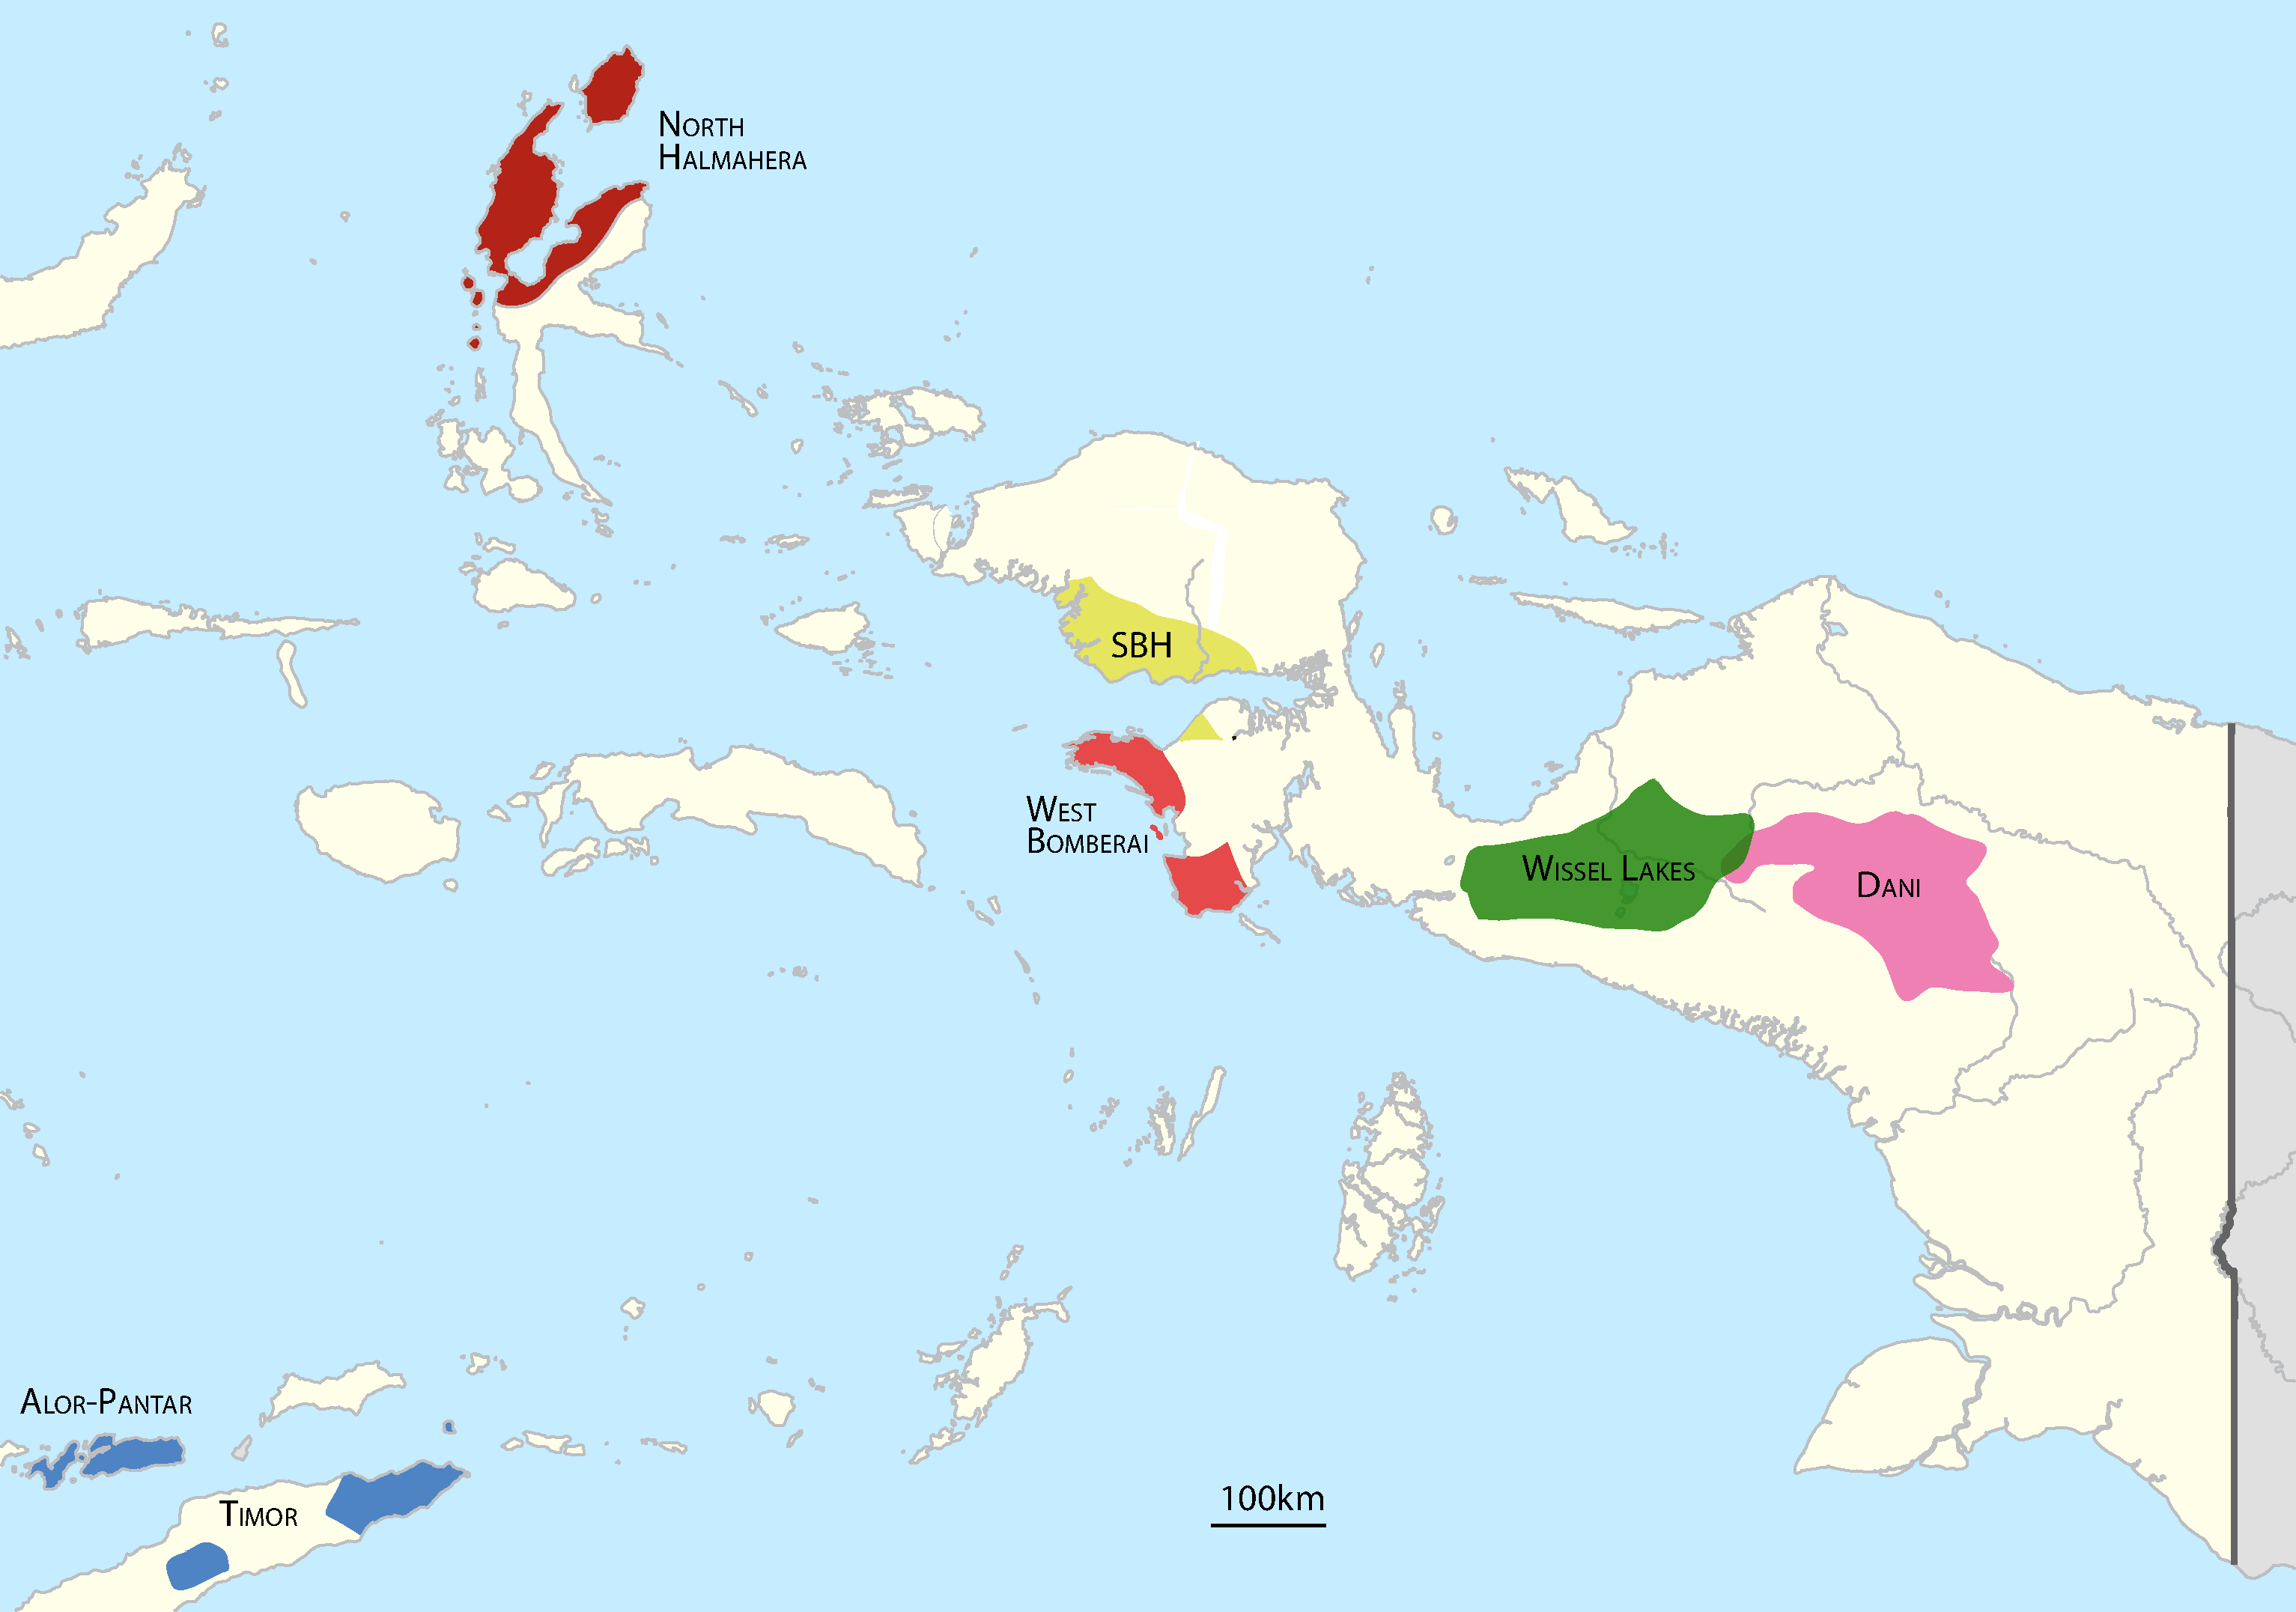
\includegraphics[width=\textwidth]{figures/Holton_ch4_fig1.pdf}
\caption{Location of Timor-Alor-Pantar languages (lower left) and putative related families discussed in this chapter}
\label{fig:4:1}
\end{figure}

In this chapter, we will consider three hypotheses about the wider relationships of the TAP family: (1) the TAP languages are related to the North Halmaheran (NH) languages\il{North Halmaheran language(s)}; (2) the TAP languages belong to the Trans-New Guinea (TNG) family\il{Trans-New Guinea language(s)} (broadly defined); and (3) the TAP languages are related to certain Papuan languages within the putative TNG family, even though the evidence linking them with TNG as a whole is indeterminate and these languages may not in fact be TNG. In order to examine the first two hypotheses we compare TAP reconstructed forms with proposed reconstructions for North Halmahera\il{North Halmaheran language(s)} and Trans-New Guinea\il{Trans-New Guinea language(s)}, respectively. In order to evaluate the third hypothesis we compare TAP reconstructions with languages from four smaller families: South Bird's Head\il{Bird's Head language(s)}; Wissel Lakes\il{Wissel Lakes language(s)}; Dani\il{Dani language(s)}; and West Bomberai\il{Bomberai language(s)}. Although each of these families has been claimed to be a part of some version of the larger Trans-New Guinea group, the composition of these smaller families is uncontroversial and thus allows us to evaluate
potential wider affiliations while remaining agnostic as to the status of Trans-New Guinea itself. Ideally, we would compare TAP to reconstructed proto-languages for each of these four families; however, given the limited historical work done on those families, we instead choose individual languages from each family for comparison with TAP. We examine each of the three hypotheses in light of recently collected data on the TAP languages, considering pronominal\is{pronoun}, typological, and lexical evidence. Finally, we conclude with a discussion of the null hypothesis that the TAP languages form a family-level isolate\is{isolate language(s)}.

The first hypothesis was suggested (and quickly discarded) by \citet{Capell1944}, who noted similarities between the Papuan languages of Timor and those of North Halmahera but initially refrained from asserting a genealogical relationship. By that time, the non-Austronesian character of the NH languages had long since been recognized, having been mentioned by \citet{VanDerAaEtAl1872} and later rigorously demonstrated by \citet{VanDerVeen1915}. \citet{Anceaux1973}, commenting on a field work report from the Pantar language Teiwa\il{Teiwa} \citep{Watuseke1973}, proposed including Teiwa and several Alor languages (Abui\il{Abui}, Wersing\il{Wersing}, Kui\il{Kui}) with Cowan's (1957) West Papuan group, which included NH.\nocite{Cowan1957}\footnote{\citet{Watuseke1973} does not identify the language as Teiwa but merely refers to it as ``a language of Pantar''. However, inspection of the data leaves no doubt that this is Teiwa.} As later formulated, Capell's (1975) West Papuan Phylum included the ``Alor-Timor'' languages. \nocite{Capell1975} In fact,
only one Alor language, Abui, was included in Capell's grouping, as Capell only belatedly became aware of the other extant Alor sources. Even with these additional data, Capell was quite conscious of the tenuous nature of the putative relationship between TAP (actually Alor-Timor) and North Halmahera\il{North Halmaheran language(s)}, particularly the lack of identifiable lexical correspondences. He thus proposed a major split between Alor-Timor (and some Bird's Head languages\il{Bird's Head language(s)}) on the one hand, and the rest of the West Papuan Phylum\il{West Papuan language(s)} on the other. Stokhof suggested connecting TAP with several languages of the Western Bird's Head of New Guinea, concluding that ``the Alor-Pantar languages form a closely related group with Cowan's West Papuan Phylum'' (1975: 26). However, the putative West Papuan languages with which Stokhof compared Alor-Pantar were later reclassified as Trans-New Guinea\il{Trans-New Guinea language(s)}, rendering this lexical evidence moot. More recently \citet{Donohue2008boundpron} has revived the NH hypothesis, based largely on pronominal\is{pronoun} evidence.

With the exception of this recent work by Donohue, the second hypothesis connecting TAP with TNG has largely supplanted the NH hypothesis in the literature. Capell's (1975) paper arguing for the NH hypothesis was published with an editorial preface noting that the TAP languages should instead be included within TNG \citep[667]{Wurm1975}. However, the accompanying paper on the TNG hypothesis in the same volume provides no data to back up this classification and instead remains skeptical as to whether TAP should be classified as Trans-New Guinea or West Papuan. In particular, the authors assert that ``whichever way they [the TAP languages] are classified, they contain strong substratum elements of the other {\dots} phyla involved'' \citep[318]{WurmEtAl1975}. Only recently have additional data been provided to support the TNG hypothesis. \citet{Pawley2001} cites lexical evidence from TAP languages in support of proto Trans-New Guinea (pTNG)\il{proto-Trans-New-Guinea} reconstructions. \citet{Ross2005} connects TAP to TNG more broadly based
on pronominal evidence. Although the evidence for the TNG hypothesis is far from overwhelming, it is today the most widely received classification, appearing for example in the most recent edition of the Ethnologue \citep{LewisEtAl2013}.

One of the challenges to finding support for the TNG hypothesis is the sheer size and diversity which exists within the family. Rather than only considering TNG as a whole, it is also useful to consider smaller families within TNG. Two proposals stand out. \citet{Reesink1996} suggests connections between TAP and the South Bird's Head family (specifically the Inanwatan language). \citet{Cowan1953} also made this connection, though he went further to group both TAP and South Bird's Head\il{South Bird's Head language(s)} within his West Papuan Phylum. A second proposal is made by \citet{Ross2005}, who considers TAP ``possibly part of a western TNG linkage'' including West Bomberai\il{Bomberai language(s)}, Wissel Lakes\il{Wissel Lakes language(s)}, and Dani\il{Dani language(s)}. As Ross suggests, this more circumscribed linkage is a group of languages descended from a dialect chain\is{dialect chain} and therefore characterized by overlapping innovations\is{innovation}. In particular, Ross notes that these languages (including the Timor languages, but excluding the Alor and Pantar languages) all show an innovative\is{innovation} metathesis\is{metathesis} of CV to VC in the first
person singular pronoun and that the TAP languages share an innovative first person plural pronoun with the West Bomberai languages (2005: 36). We are not aware of any serious proposals connecting TAP to Papuan languages outside NH\il{North Halmaheran language(s)} (and the West Papuan Phylum\il{West Papuan language(s)}) and TNG\il{Trans-New Guinea language(s)}.

The possibility that the TAP languages form a family-level isolate\is{isolate language(s)} not demonstrably related to other Papuan languages was actually suggested by Capell, who concluded:

\begin{quote}
Neither are the `Papuan' languages outside New Guinea, in the Solomons, New Britain, Halmahera or Timor related to each other or to those of New Guinea. At least it cannot be assumed that any two are related{\dots}. (1944: 313)
\end{quote}

However, this null hypothesis has not, to our knowledge, been given serious consideration in the literature. We return to this point in our conclusion ({\S}~\ref{sec:4:6}). In the meantime we evaluate the first two hypotheses in light of the typological evidence ({\S}~\ref{sec:4:2}), pronominal evidence ({\S}~\ref{sec:4:3}), and lexical evidence ({\S}~\ref{sec:4:4}). Evidence for the third hypothesis linking the TAP family with individual languages in Papua is considered in {\S}~\ref{sec:4:5}.

\section{Typological evidence}\label{sec:4:2}
Given that typological features can easily cross genealogical boundaries, typological evidence for genealogical relationships should be approached with caution. \citet{KlamerEtAl2008} argue that the region under consideration here---spanning from TAP to NH to New Guinea---is part of the East Nusantara linguistic area which shares a number of typological features in spite of genealogical differences among languages. Moreover, these features are not particularly unique and hence do not provide any special proof of genealogical connection in the sense of \citet{Meillet1967}. On the other hand, we feel that a volume on the Alor-Pantar languages would not be complete without a discussion of how the typological profile of the family relates to those of the surrounding Papuan languages. Nonetheless, we find little evidence for shared typological features between TAP and either the NH\il{North Halmaheran language(s)} or TNG families\il{Trans-New Guinea language(s)}. In this section we provide examples contrasting the typological profiles of these families, considering phonology ({\S}~\ref{sec:4:2.1}), morphology ({\S}~\ref{sec:4:2.2}), and syntax ({\S}~\ref{sec:4:2.3}).

\subsection{Phonology}\label{sec:4:2.1}
\citet{Foley1998} suggests two typically Papuan phonological features: the presence of a single liquid phoneme and the presence of pre-nasalized stops. Neither of these putative Papuan phonological features is found in proto-Timor-Alor-Pantar (pTAP), which had at least two liquids and lacks pre-nasalized stops. The pTAP consonant inventory (based on Chapter 3), is shown in Table \ref{tab:4:1}.


\begin{table}[h]
\centering
\caption{pTAP consonants (based on Chapter 3)} 
\label{tab:4:1}
\begin{tabular}{>{\scshape}lccccc}
\mytopline
  &\textsc{labial}&\textsc{alveolar}&\textsc{palatal}&\textsc{velar}&\textsc{glottal}\\
\midrule  
{voiceless stops}& p & t && k &\\
{voiced stops}& b & d && g &\\
{nasals}& m & n &&&\\
{fricatives}&& s &&& h \\
{glides}& w && j &&\\
{liquids}&& l r\footnotemark{} &&&\\
\mybottomline
\end{tabular}
\end{table}

\footnotetext{\label{fn:4:4}\citet{SchapperEtAlTVtimor} note that there are three correspondence sets between AP on the one hand, and Timor-Kisar, on the other, and so they reconstruct a third liquid *R, but they do not speculate about the phonetic value of *R. Since none of the modern TAP languages has more than two liquids, we believe that the proto-language had just two liquids, and that the third correspondence set should be attributed to either *r or *l, with some as yet to be identified conditioning. }
Nor are these features present in proto-North Halmahera (pNH)\ilt{proto-North-Halmahera}, shown in Table \ref{tab:4:2}.




\begin{table}[t]
\centering
\caption{pNH\ilt{proto-North-Halmahera} consonants \citep[after][]{Wada1980}}
\label{tab:4:2}
\begin{tabular}{>{\scshape}lccccc}
\mytopline
&\textsc{labial}&\textsc{alveolar}&\textsc{retroflex}&\textsc{velar}&\textsc{glottal}\\
\midrule  
{voiceless stops}& p & t && k &\\
{voiced stops}& b & d & {\textrtaild} & g &\\
{nasals}& m & n && {\ng} &\\
{fricatives}&& s &&& h \\
{glides}& w &&&&\\
{liquids}&& l & r &&\\
\mybottomline
\end{tabular}
\end{table}

On the other hand, both pre-nasalized stops and a single liquid phoneme are found in pTNG\il{proto-Trans-New-Guinea}. Additionally, in contrast to either pTAP\il{proto-Timor Alor Pantar} or pNH\il{proto-North-Halmahera}, pTNG\il{proto-Trans-New-Guinea} contains only a single fricative (Table \ref{tab:4:3}).


\begin{table}[h]
\centering
\caption{pTNG consonants \citep{Pawley1995,Pawley2001}}
\label{tab:4:3}
\begin{tabular}{>{\scshape}lccc}
\mytopline
 &\textsc{labial}&\textsc{apical}&\textsc{velar}\\
\midrule  
{oral stops}& p & t\footnotemark{} & k \\
{prenasalized stops}& mb & nd & {\ng}g \\
{nasals}& m & n & {\ng} \\
{fricatives}&& s &\\
{glides}& w & y &\\
{liquid}&& l &\\
\mybottomline
\end{tabular}
\end{table}

\footnotetext{Note that the pTNG\ilt{proto-Trans-New-Guinea} apical stop *t may have had a flap or trill allophone \citep[273]{Pawley2001}.}
In many respects, these three consonant inventories are similar. Each contains two sets of stops. In pTAP\il{proto-Timor Alor Pantar} and pNH\il{proto-North-Halmahera}, the distinction between the two sets is voicing, with one voiced set and one voiceless set. In pTNG\il{proto-Trans-New-Guinea} the distinction is between oral and pre-nasalized. It is plausible that the pTNG\il{proto-Trans-New-Guinea} pre-nasalized stops developed into the pTAP\il{proto-Timor Alor Pantar} voiced stops. Nevertheless, considering just the four phonological features discussed above we find greater similarity between TAP and NH\il{North Halmaheran language(s)} than between TAP and TNG\il{Trans-New Guinea language(s)}, as summarized in Table \ref{tab:4:4}.



\begin{table}[t]
\centering
\caption{Summary of TAP, TNG\il{Trans-New Guinea language(s)} and NH\il{North Halmaheran language(s)} phonological features}
\label{tab:4:4}
\begin{tabular}{>{\scshape}lccc}
\mytopline
&TAP&TNG&NH\\
\midrule
pre-nasalized stops& - & {\checkmark} & - \\
single liquid& - & {\checkmark} & - \\
uvular consonant& {\checkmark} & - & - \\
single fricative& - & {\checkmark} & - \\
\mybottomline
\end{tabular}
\end{table}


\subsection{Morphology} \label{sec:4:2.2}
Among the few typologically distinctive morphological features of the TAP languages is the presence of pronominal\is{pronoun} indexing of the patient-like argument of a transitive verb (P) via a pronominal prefix (see Chapter 10). Reflexes of a P prefix are widely distributed across the family and can be reconstructed to pTAP. These prefixes generally have the same form as those which index possessors\is{possession} on nouns, as in the Teiwa\il{Teiwa} example in \REF{ex:4:1}, where the third singular prefix on the verb indexes the third singular P argument, while the first singular prefix on the noun `child' indexes the possessor.

\ea% 1
\label{ex:4:1}
\langinfo{Teiwa}{AP}{\citealt[159]{Klamer2010grammar}} \\
\gll  Name, ha{\textglotstop}an n-oqai g-unba{\textglotstop}. \\
  Sir \textsc{2sg} \textsc{1sg}-child \textsc{3sg}-meet  \\
\glt `Sir, did you see (lit. meet) my child?'
\z




However, P prefixes are in general not obligatory in TAP, and the conditions on pronominal alignment\is{alignment} vary considerably among the individual languages of the family \citep[Chapter 10]{FeddenEtAl2013}. For example, Bunaq\il{Bunaq} (Timor) does not use pronominal prefixes to index inanimate P arguments. In example \REF{ex:4:2}, there is no prefix on the verb because the P argument \textit{zo} `mango' is inanimate. In example \REF{ex:4:3}, in contrast, the verb takes a third person prefix which indexes \textit{zap} `dog'.

\ea% 2
\label{ex:4:2}
\langinfo{Bunaq}{Timor}{\citealt[122]{Schapper2009}} \\
\gll  Markus zo poi \\
   Markus mango  choose \\
\glt `Markus chose a mango.'
\z





\ea% 3
\label{ex:4:3}
\langinfo{Bunaq}{Timor}{\citealt[122]{Schapper2009}} \\
\gll  Markus zap go-poi \\
    Markus dog \textsc{3}-choose\\
\glt `Markus chose a dog.'
\z




In the AP language Abui, alignment is semantic, and most non-volitional arguments are marked with pronominal\is{pronoun} prefixes, including non-volitional S arguments \citep[Chapter 10]{FeddenEtAl2013}. In \REF{ex:4:4} the sole argument is volitional, so there is no marking on the verb. In \REF{ex:4:5} the first person undergoer is non-volitional and is indexed on the verb with the prefix \textit{no-.} Likewise, in \REF{ex:4:6} the verb \textit{wel }`pour' takes the third person prefix \textit{ha-} because the undergoer \textit{Simon} is non-volitional. Finally, we see in \REF{ex:4:7} that even the sole argument of the verb can be indexed with a prefix if it is non-volitional\is{volitionality}.

\ea% 4
\label{ex:4:4}
\langinfo{Abui}{AP}{\citealt[80.171]{Kratochvil2007}} \\
\gll  Na sei. \\
  \textsc{1sg} come.down \\
\glt `I come down.'
\z





\ea% 5
\label{ex:4:5}
\langinfo{Abui}{AP}{\citealt[80.171]{Kratochvil2007}} \\
\gll  Simon no-dik. \\
  Simon \textsc{1sg}-tickle  \\
\glt `Simon is tickling me.'
\z





\ea% 6
\label{ex:4:6}
\langinfo{Abui}{AP}{\citealt[80.171]{Kratochvil2007}} \\
\gll  Na Simon ha-wel. \\
  \textsc{1sg} Simon 3-pour  \\
\glt `I washed Simon.'
\z





\ea% 7
\label{ex:4:7}
\langinfo{Abui}{AP}{\citealt[80.171]{Kratochvil2007}} \\
\gll  No-lila. \\
  \textsc{1sg}-be.hot  \\
\glt `I am hot.'
\z





A few TAP languages also permit indexing of both A and P arguments via pronominal\is{pronoun} prefixes. In such cases, the prefix paradigms for each argument are identical.

\ea% 8
\label{ex:4:8}
\langinfo{Western Pantar}{AP}{\citealt{Holton2010person}} \\
\gll  Ke'e pi-ga-ussar. \\
   fish \textsc{1pl-3sg}-catch \\
\glt `We're catching fish.'
\z





The North Halmaheran languages\il{North Halmaheran language(s)} also index P arguments on the verb, and as in TAP, the conditions on pronominal\is{pronoun} indexing vary considerably across different languages in the family \citep{Holton2008}. However, pronominal indexing in NH languages differs in several respects from that found in TAP. First, not just P but also A is referenced on the verb in NH. Second, for most NH languages pronominal indexing is obligatory. Third, unlike TAP languages, the forms of A and P pronominal prefixes differ from each other in NH. That is, A and P arguments are marked by distinct paradigms, and this holds for both pronominal prefixes as well as independent pronouns. The Tobelo example in \REF{ex:4:9} illustrates these properties.

\ea% 9
\label{ex:4:9}
\langinfo{Tobelo}{NH}{\citealt{Holton2003}} \\
\gll  (Ngohi) t-i-ngoriki. \\
    (\textsc{1sg}) \textsc{1sg-3sg.m}-see\\
\glt `I see him.'
\z





Moreover, in NH languages the order of verbal referents is fixed as actor-undergoer, while for TAP languages which permit two pronominal prefixes, the order may in some cases be reversed as undergoer-actor, as in \REF{ex:4:10}.

\ea% 10
\label{ex:4:10}
\langinfo{Western Pantar}{AP}{Holton fieldnotes} \\
\gll  gai ya me ga-na-asang \\
 \textsc{3poss} road \textsc{loc} \textsc{3sg-1sg}-say  \\
\glt `I will tell him the way.' (lit., `I will him about his road.')
\z

 



Indexing of P arguments is also a prominent feature of verbs in Trans-New Guinea languages\il{Trans-New Guinea language(s)}. Verbs with P arguments indexed via prefixes are found for example in the Finisterre-Huon family\il{Finisterre-Huon language(s)}, and P-marking prefixes can be reconstructed at the level of pTNG\il{proto-Trans-New-Guinea} \citep{Suter2012}. Indexing of P arguments is illustrated in \REF{ex:4:11} with data from Fore, where the first person singular object is indicated with a verbal prefix.

\ea% 11
\label{ex:4:11}
\langinfo{Fore}{TNG}{\citealt[107]{Scott1978}} \\
\gll  N\'ae na-ka-y-e. \\
  1\textsc{sg} \textsc{1sg.und}-see-\textsc{3sg.act-decl}  \\
\glt `He sees me.'
\z





In contrast to both TAP and NH languages\il{North Halmaheran language(s)}, pTNG\il{proto-Trans-New-Guinea} indexed subjects (both A and S) via suffixes, not prefixes \citep{Foley2000}. However, subject prefixes are not unknown in TNG languages\il{Trans-New Guinea language(s)}. Foley cites Marind\il{Marind} as an example of a Papuan language with both subject and object prefixes, noting that ``Marind is the only Papuan language I know which consistently exhibits A-U-V order'' \citeyearpar[138]{Foley1986}.

\ea% 12
\label{ex:4:12}
\langinfo{Marind}{TNG}{\citealt{Drabbe1955}, cited in \citealt[138]{Foley1986}} \\
\gll  A-na-kipraud. \\
   3\textsc{sg.subj-1sg.obj-}tie \\
\glt `He ties me.'
\z





While the Marind example in \REF{ex:4:12} may not be typical for TNG languages, it certainly shows much affinity with pronominal indexing patterns in both TAP and NH languages.

The TAP languages exhibit preposed possessor constructions, a typically Papuan feature, at least for East Nusantara \citep{KlamerEtAl2008}. The possessor precedes the possessum, whether the possessor is expressed as a full noun phrase \REF{ex:4:13} or just with a pronoun \REF{ex:4:14}.


\ea% 13
\label{ex:4:13}
\langinfo{Western Pantar}{AP}{Holton fieldnotes} \\
\gll  yabbe si gai bla \\
   dog that \textsc{3sg.poss} house \\
\glt `the dog's house'
\z





\ea% 14
\label{ex:4:14}
\langinfo{Western Pantar}{AP}{Holton fieldnotes} \\
\gll  nai bla \\
  \textsc{1sg.poss} house \\
\glt `my house'
\z





NH languages exhibit a similar pattern of possessor-possessum\is{possession} order, as in the Tobelo examples below.

\ea% 15
\label{ex:4:15}
\langinfo{Tobelo}{NH}{\citealt{Holton2003}} \\
\gll  o-kaho ma-tau \\
   \textsc{nm}-dog \textsc{nm}-house\\
\glt `the dog's house'
\z





\ea% 16
\label{ex:4:16}
\langinfo{Tobelo}{NH}{\citealt{Holton2003}} \\
\gll  ahi-tau \\
 \textsc{1sg.poss}-house  \\
\glt `my house'
\z





The order possessor-possessum\is{possession} is also found widely among TNG languages\il{Trans-New Guinea language(s)}, as illustrated by the Enga and Mian examples below.

\ea% 17
\label{ex:4:17}
\langinfo{Enga}{TNG}{\citealt[264]{Foley1986}} \\
\gll  namba-ny\'a men\'a \\
 \textsc{1sg-poss} pig  \\
\glt `my pig'
\z





\ea% 18
\label{ex:4:18}
\langinfo{Mian}{TNG}{\citealt[217]{Fedden2011}} \\
\gll  \=ob imak \\
   \textsc{2sg.f.poss} husband\\
\glt `your husband'
\z





The order possessum-possessor is also found in many TNG languages, particularly with inalienable\is{alienability} nouns, as illustrated by the following examples from Fore and Barai.


\ea% 19
\label{ex:4:19}
\langinfo{Fore}{TNG}{\citealt[31]{Scott1978}} \\
\gll  yaga-nene \\
   pig-\textsc{1sg.poss} \\
\glt `my pig'
\z





\ea% 20
\label{ex:4:20}
\langinfo{Barai}{TNG}{\citealt{Olson1981}, cited in \citealt{Foley1986}} \\
\gll  e n-one \\
   person \textsc{1sg-poss} \\
\glt `my people'
\z





A distinction between alienable\is{alienability} and inalienable possession\is{possession} is considered a typical Papuan feature, and TAP languages share this feature. While TAP languages vary in exactly how they realize this distinction, Western Pantar\il{Western Pantar} is typical in realizing this distinction in the possessive pronouns. In Western Pantar the third person singular inalienable\is{alienability} form is \textit{ga-} rather than \textit{gai-}, as in \REF{ex:4:21}.

\ea% 21
\label{ex:4:21}                                
\langinfo{Western Pantar}{AP}{Holton fieldnotes} \\
\gll  ga-uta  (*gai-) \\
  \textsc{3sg.inal}-foot  \textsc{(3sg.alien-)} \\
\glt `his/her/its foot'
\z
 
Many of the TNG languages\il{Trans-New Guinea language(s)} also share this distinction. In Inanwatan\il{Inanwatan}, alienably possessed\is{possession} nouns take independent pronouns\is{pronoun}, like \textit{tig\'aeso} in \REF{ex:4:22}, while inalienably possessed nouns take pronominal prefixes, like \textit{na- }in \REF{ex:4:23}.

\ea% 22
\label{ex:4:22}
\langinfo{Inanwatan}{South Bird's Head}{\citealt[29, 30]{DeVries2004}}\footnote{The acute accent indicates lexical stress, which is distinctive in Inanwatan.})\\
\gll  tig\'ae-so suq\'ere \\
  \textsc{3sg.f}-\textsc{m} sago.\textsc{m} \\
\glt `her sago'
\z





\ea% 23
\label{ex:4:23}
\langinfo{Inanwatan}{South Bird's Head}{\citealt[29, 30]{DeVries2004}}\\
\gll  n\'a-wiri \\
 \textsc{1sg}-belly.\textsc{m}  \\
\glt `my belly'
\z





While NH languages\il{North Halmaheran language(s)} also have obligatorily possessed nouns, these languages lack a distinct inalienable possession construction. In particular, in NH languages the same possessive construction is used regardless of whether the noun is obligatorily possessed or not. In Tobelo\il{Tobelo} obligatorily possessed nouns such as \textit{lako }`eye' \REF{ex:4:24} use the same possessive strategy as non-obligatorily possessed nouns such as \textit{tau }`house' \REF{ex:4:16}.



\ea% 24
\label{ex:4:24}
\langinfo{Tobelo}{NH}{Holton fieldnotes} \\
\ea
  \gll ma-lako \\
    \textsc{nm}-eye  \\
\glt `eye' 
    \ex
    \gll o-kaho ma-lako \\
    \textsc{nm}-dog \textsc{nm}-eye\\
\glt `the dog's eye'
    \ex
    \gll ahi-lako\\
    \textsc{1sg.poss}-eye\\
\glt `my eye'
  \z
\z

The morphological features for TAP, TNG\il{Trans-New Guinea language(s)}, and NH\il{North Halmaheran language(s)} are summarized in Table \ref{tab:4:5}.



\begin{table}[h]
\centering
\caption{Summary of TAP, TNG, and NH morphological features}
\ilt{North Halmaheran language(s)}\ilt{Trans-New Guinea language(s)} 
\label{tab:4:5}
\ist{pronoun} \ist{possession}\ist{alienability}
\begin{tabular}{lccc}
\mytopline
& TAP & TNG& NH \\
\midrule
pronominal object prefixes (P)& {\checkmark} & {\checkmark} & {\checkmark} \\
pronominal subject affixes (A/S)& ({\checkmark}) & {\checkmark} & {\checkmark} \\
preposed possessors& {\checkmark} & ({\checkmark}) & {\checkmark} \\
alienable/inalienable distinction& {\checkmark} & {\checkmark} & - \\
\mybottomline
\end{tabular}
\end{table}



\subsection{Syntax} \label{sec:4:2.3}
The TAP languages, like most NH and TNG \citep{Foley2000} languages, are right-headed\is{right-headed} and verb-final\is{verb-final}.


\ea% 25
\label{ex:4:25}
\langinfo{Adang}{AP}{\citealt[121]{Haan2001}} \\
\gll  Pen ti mat{\textepsilon} s{\textepsilon}l al{\textopeno} {\textglotstop}a-b{\textopeno}{\textglotstop}{\textopeno}i. \\
   John tree big \textsc{clf} two 3\textsc{obv}-cut \\
\glt `John cut the two big trees.'
\z





\ea% 26
\label{ex:4:26}
\langinfo{Tobelo}{NH}{\citealt{Holton2003}} \\
\gll  Ngohi o-pine t-a-ija. \\
 \textsc{1sg} \textsc{nm}-rice \textsc{1sg-3sg}-buy  \\
\glt `I bought the rice.'
\z






\ea% 27
\label{ex:4:27}
\langinfo{Mian}{TNG}{\citealt[344]{Fedden2011}} \\
\gll  N\'e imen-o wen-b-i=be. \\
 \textsc{1sg} taro-\textsc{nc.pl} eat-\textsc{ipfv-1sg.subj=decl}  \\
\glt `I am eating taro.'
\z





Also like the NH languages and the TNG languages, the TAP languages have postpositions, as in the Bunaq\il{Bunaq} example \REF{ex:4:28}, where the locative postposition\is{adposition} \textit{gene} follows its nominal complement \textit{reu} `house'.





 
\ea% 28
\label{ex:4:28}
\langinfo{Bunaq}{Timor}{\citealt[104]{Schapper2009}} \\
\gll   neto  reu  gene  mit\\ 
\textsc{1sg}  house  \textsc{loc}  sit\\  
\glt `I sit at home.'  \\

\z
 




In many TAP languages, however, the postpositions\is{adposition} display verbal properties, as in \REF{ex:4:29}, where the postposition/verb \textit{mi} `(be) in' is modified by an aspectual marker\is{aspect}.


\ea% 29
\label{ex:4:29}
\langinfo{Adang}{AP}{Robinson fieldnotes} \\
\gll  {\textglotstop}am{\textopeno} nu meja far mi eh. \\
   cat one table below be.in \textsc{prog} \\
\glt `A cat is beneath a table.'
\z





Another typically Papuan feature in East Nusantara languages is the presence of clause-final negation\is{negation} \citep{KlamerEtAl2008}. This feature is indeed found in TAP languages \REF{ex:4:30}, though in NH languages\il{North Halmahera language(s)} the negator morpheme just follows the verb root rather than occurring in absolute final position \REF{ex:4:31}.


\ea% 30
\label{ex:4:30}
\langinfo{Western Pantar}{AP}{Holton fieldnotes} \\
\gll  Gang ke'e na wang yawang kauwa. \\
  \textsc{3sg}.act meat eat exist agree \textsc{neg} \\
\glt `He doesn't like to eat meat.'
\z






\ea% 31
\label{ex:4:31}
\langinfo{Tobelo}{NH}{\citealt{Holton2003}} \\
\gll  Wo-honenge-ua-ahi. \\
 \textsc{3sg.act}-die-\textsc{neg-ipfv}  \\
\glt `He is not yet dead.'

\z

 


One notable syntactic feature absent from TAP is clause-chaining\is{clause-chaining}, which is one of the most distinctive features of Papuan languages in general and is particularly associated with TNG languages\il{Trans-New Guinea language(s)} (\citealt[175]{Foley1986}, \citealt{Roberts1997}). Clause-chaining is also absent from NH languages\il{North Halmaheran language(s)}. However, while clause-chaining may be one of the key distinguishing features of Papuan languages, it is important to note that this feature is completely absent from some TNG languages, such as Marind\il{Marind}.



In general, syntactic features do not distinguish the TAP languages from TNG or NH (Table \ref{tab:4:6}).

\begin{table}[h]
\centering
\caption{Summary of TAP, TNG, and NH syntactic features}
\label{tab:4:6}
\begin{tabular}{llll}
\mytopline
& TAP & TNG & NH \\
\midrule
verb-final& {\checkmark} & {\checkmark} & {\checkmark} \\
postpositions& {\checkmark} & {\checkmark} & {\checkmark} \\
clause final negation& {\checkmark} & {\checkmark} & {\checkmark} \\
clause chaining& - & ({\checkmark}) & - \\
\mybottomline
\end{tabular}
\end{table}

While the TAP languages share a number of morphological and syntactic features with TNG and NH languages, these features are typologically common, may be interrelated (such as verb-final syntax and postpositions\is{adposition}), and they may be indicative of a linguistic area \citep{KlamerEtAl2008}. We therefore do not find the typological evidence convincing of genealogical relationship.

\section{Pronominal\ist{pronoun} evidence} \label{sec:4:3}
When combined with other lines of evidence, homologous pronominal paradigms can provide strong support for proposals of genealogical relatedness. However, the use of pronominal paradigms as the \textit{sole }evidence for genealogical relatedness has been repeatedly questioned in the literature \citep[cf.][]{CampbellEtAl2008}. Pronominal paradigms were an important basis for the development of the Trans-New Guinea\il{Trans-New Guinea language(s)} hypothesis \citep{WurmEtAl1975}, and pronouns have continued to play a starring role in attempts to subgroup the TNG languages \citep{Ross2005,Ross2006}.\footnote{As originally formulated, the Trans New Guinea hypothesis linked Central and South New Guinea languages with the Finisterre-Huon languages based not on pronominal evidence but on lexical similarities \citep{McElhanonEtAl1970}.} In this section we consider the strength of the pronominal evidence in evaluating the Trans-New Guinea and North Halmaheran\il{North Halmaheran language(s)} hypotheses.
 

Since the full pronominal paradigm has not been reconstructed for pTAP, we consider the reconstructed pAP pronouns here. They are shown in Table \ref{table_pronouns}, together with the pTNG\il{proto-Trans-New-Guinea} \citep{Ross2005} and pNH\il{proto-North-Halmahera} \citep{Wada1980} pronouns. Note that North Halmaheran pronouns are reconstructed in two forms corresponding to actor (``subject'') and undergoer (``object'').




\begin{table}[h]
\centering
\begin{tabular}{lllp{2cm}p{2cm}}
\mytopline
&  pAP\ilt{proto-Alor-Pantar} &   pTNG\ilt{proto-Trans-New-Guinea} & \multicolumn{2}{c}{  pNH\ilt{proto-North-Halmahera}}\hspace{1cm} \\
&&& \rm \textsc{act} & \rm \textsc{und}\\ 
\midrule
\textsc{1sg}& *na- & *na & *to- & *si- \\ 
\textsc{2sg}& *(h)a- & *{\ng}ga & *no- & *ni- \\ 
\textsc{3sg}& *ga- & *ua, *(j)a & *mo- (\textsc{fem}) \newline *wo- (\textsc{mas}) \newline *i- (\textsc{neu}) 
 
 & *mi- (\textsc{fem}) \newline *wi- (\textsc{mas}) \newline *ja- (\textsc{neu})  \\ 
 
\textsc{1pl.incl}& *pi- & *nu, *ni & *po- & *na- \\ 
\textsc{1pl.excl}& *ni- & - & *mi- & *mi- \\ 
\textsc{1distr}& *ta- & - & - & -\\ 
\textsc{2pl}& *(h)i- & *nja, *{\ng}gi & *ni- & *ni- \\ 
\textsc{3pl}& *gi- & *i & *jo- & *ja- \\ 

\mybottomline
\end{tabular}

\caption{pAP, pTNG, and pNH pronouns\ist{pronoun}}
\label{table_pronouns}

\label{tab:4:7}
\end{table}


Several structural differences are noticeable between these pronoun sets. First, AP and NH show an inclusive/exclusive distinction in first person plural\is{plurality} which is not found in TNG. This has been argued to be an areal feature resulting from Austronesian\il{Austronesian language(s)} influence \citep{KlamerEtAl2008}. Second, NH but not AP or TNG distinguish gender in third person pronouns. Third, a distributive \is{distributive} pronoun is found only in AP.

We consider first the TNG pronouns. The pTNG pronominal reconstructions provide what some consider to be the strongest support for the genealogical connection between AP and TNG\il{Trans-New Guinea language(s)} \citep{Ross2005}. Both pTNG and pAP show a paradigmatic distinction between \textit{a} in the singular and \textit{i} in the plural\is{plurality}. However, the correspondence is problematic due to the mismatch between the second and third person pronouns. Proto-TNG shows velar consonants in the second person forms, while pAP shows velar consonants in the third person forms. It has been suggested that the pTNG second person pronouns could have developed into the pAP second person pronouns by lenition of pTNG *{\ng}g {\textgreater} *g {\textgreater} *k {\textgreater} h. While this is possible, we find stronger evidence that the pTNG prenasalized obstruents should correspond to the pAP voiced stops (see {\S}~\label{sec:4:4.2}), if indeed the two are related at all.

Another possible scenario connecting these two paradigms is to posit a flip-flop between the second and third person pronouns, as in \REF{ex:4:32}. As far as we are aware, such an inversion scenario was first proposed by \citet{DonohueEtAl2007}.

\ea% 32
\label{ex:4:32}
   {\upshape Putative flip-flop between second and third person pronouns\ist{pronoun}  }\\
\begin{tabular}{>{\rm}l@{{\textgreater}}>{\rm}l}
pTNG\ilt{proto-Trans-New-Guinea} *{\ng}ga `\textsc{2sg}'  & pAP *ga- `\textsc{3sg}'\\
pTNG *{\ng}gi `\textsc{2pl}'  & pAP\ilt{proto-Alor-Pantar} *gi- `\textsc{3pl}' \\
pTNG *(y)a `\textsc{3sg}'     & pAP *(h)a- `\textsc{2sg}'\\
pTNG *i `\textsc{3pl}'        & pAP *(h)i- `\textsc{2pl}'\\
\end{tabular}
\z


This leaves only the fricative in the pAP second person forms unexplained, but external evidence from the Timor languages suggests that perhaps the pAP second person forms should be vowel initial (i.e., pAP *a `\textsc{2sg'} and *i `\textsc{2pl'}). While it is not impossible that the pAP pronouns descend from the pTNG pronouns in this way, connecting the two requires us to posit a flip which makes the correspondence much less striking.

The putative correspondence between the pAP and pTNG pronouns leaves at least one AP form unexplained: the AP distributive *ta- has no correspondent form in TNG\il{Trans-New Guinea language(s)}. \citet{Donohue2008boundpron} posits a connection between the AP distributive and the pNH\il{proto-North-Halmahera} first-singular active form *to-. According to this hypothesis the resemblance between the AP distributive and the pNH first-singular active is evidence not of a genealogical relationship but rather a borrowing\is{borrowing} relationship within a contact area encompassing the Bomberai Peninsula and South Bird's Head region. The semantic plausibility of this connection is based on an analysis of *ta- as the minimal 1/2-person pronoun in a minimal-augmented system \citep{Donohue2007phonological}. However, the augmented counterpart is filled anomalously by *pi-, rather than the expected *ti-, though pAP *pi- does show striking semantic and structural similarity with pNH first person inclusive *po-. Yet in the modern Alor-Pantar languages, reflexes of *ta-, where they exist, have a clear distributive
function. For example, compare the Adang first person plural inclusive (33a) with the distributive (33b).


\ea% 33
\label{ex:4:33}
\langinfo{Adang}{AP}{\citealt{Haan2001}} \\
\ea
\gll Sa pi-ri b{\textepsilon}h. \\
    \textsc{3sg} \textsc{1pl.incl-acc} hit \\
\glt `She hit (all of) us.' 
  \ex 
  \gll Sa ta-ri b{\textepsilon}h \\
  \textsc{3sg} \textsc{distr-acc} hit \\
\glt `She hit each one of us.'
  \z
\z

The distributive function is expressed quite differently in NH languages\il{North Halmaheran language(s)}. In Tobelo the distributive is expressed with the verb prefix \textit{koki-} \REF{ex:4:34} rather than with a pronoun\is{pronoun}.


\ea% 34
\label{ex:4:34}
\langinfo{Tobelo}{NH}{\citealt{Holton2003}} \\
\gll  ma-homoa yo-koki-honeng-oka  \\
   \textsc{nm}-other \textsc{3pl-distr}-die-\textsc{prf} \\
\glt `Each of the others died.'
\z





The AP distributive prefix is extra-paradigmatic: it does not show the vowel grading found in the other prefixes; and  related independent pronouns\is{pronoun} are either absent or of limited distribution. This suggests that the pAP\il{proto-Alor-Pantar} distributive has a distinct history from that of the other pAP pronominal forms, and that the resemblance between pNH\il{proto-North-Halmahera} *to `\textsc{1sg}' and pAP *ta `\textsc{1pl.dist}' is coincidental.

The structural features of the pronominal systems are compared in Table \ref{tab:4:table_pronominal_features}. It is apparent that the AP pronominal system as a whole has relatively little in common with TNG\il{Trans-New Guinea language(s)} and NH\il{North Halmaheran language(s)}.



\begin{table}[h]
\centering
\caption{Summary of AP, TNG\ilt{Trans-New Guinea language(s)}, and NH\ilt{North Halmaheran language(s)} pronominal\ist{pronoun}}
\label{tab:4:table_pronominal_features}
\begin{tabular}{llll}
\mytopline
& AP & TNG & NH \\
\midrule
 {}[a] singular, [i] plural& {\checkmark} & {\checkmark} & - \\
distributive pronoun& {\checkmark} & - & - \\
inclusive/exclusive distinction& {\checkmark} & - & {\checkmark} \\
gender distinction& - & - & {\checkmark} \\
\mybottomline
\end{tabular}
\end{table}

Given the rather speculative nature of the second-third person inversion hypothesis, the pronominal evidence does not provide very strong support for either the TNG or NH hypothesis. Nevertheless, the formal correspondence in first-person forms between AP and TNG provide tentative support for a connection between TAP and TNG.

\section{Lexicon} \label{sec:4:4}
When combined with evidence from morphological paradigms, such as pronouns, lexical evidence based on regular sound correspondences is usually considered to be compelling evidence for positing genealogical relationships between languages. Unfortunately, very little in the way of lexical evidence had been previously considered in assessing the wider genealogical relationships of the TAP languages before  \citet{RobinsonEtAl2012reassessing}. We consider first the lexical evidence for the NH hypothesis and then the lexical evidence for the TNG\il{Trans-New Guinea language(s)} hypothesis.

\subsection{Lexical evidence for the NH hypothesis}
The lexical evidence for a connection between TAP and NH languages\il{North Halmaheran language(s)} is not particularly convincing. In a list of 92 basic vocabulary terms, Capell identifies 11 which seem to show ``common roots'' with AP languages (1975: 685). Capell did not include data from Pantar languages and hence refers to this family as Alor-Timor. In many cases Capell's proposed Alor-Timor forms differ from the pTAP\il{proto-Timor Alor Pantar} reconstructions in Chapter 3. This may be due in some cases to excessive reliance on Timor forms. In Table \ref{tab:4:9} we list Capell's Alor-Timor alongside updated pTAP forms. Where available, we use pTAP reconstructions (Chapter 3), but if no pTAP reconstruction exists, then we show lower-level reconstructions or forms from individual languages. In two cases Capell's `Alor-Timor' form is quite different from the updated TAP form. Capell's \textit{hele} `stone' differs from pTAP *war but compares to Bunaq\il{Bunaq} (Timor) \textit{hol. }We have no reconstruction for `cut' in pTAP, but Capell's form \textit{uti }compares with Makalero\il{Makalero} (Timor)
 \textit{teri. }Three of Capell's NH reconstructions are also problematic; we have noted these problems in the last column in Table \ref{tab:4:9}. Capell's NH *utu `fire' should clearly be *uku, perhaps a typographical error. Capell's *helewo `stone' is found in Tobelo but does not reconstruct to NH. We are not able to identify Capell's *hate `tree'; the form *gota reconstructs for the family.




\begin{sidewaystable}\centering
\caption[Comparison of Capell's TAP and NH\ilt{North Halmaheran language(s)}, with modern TAP and NH reassessments]{Comparison of Capell's TAP and NH\ilt{North Halmaheran language(s)}, with modern TAP and NH reassessments{\footnotemark}}
\label{tab:4:9}
\begin{tabular}{l>{\it}lp{7.5cm}p{2cm}p{2.3cm}}
\mytopline
&\rm TAP (Capell)&\rm TAP (revised)&\rm NH\ilt{North Halmaheran language(s)} (Capell)&\rm NH (revised)\\
\midrule  
`bitter'&malara&proto-Alor\ilt{proto-Alor} (but not pAP\ilt{proto-Alor-Pantar} or pTAP\ilt{proto-Timor Alor Pantar}) *makal&*mali&\\
`cold'&palata&Abui\ilt{Abui}, Kui\ilt{Kui} \textit{palata}&*malata&\\
`cry out'&(k)ole&Nedebang\ilt{Nedebang} \textit{uwara}, Sawila\ilt{Sawila} \textit{kawa},
\par Makasae\ilt{Makasae} \textit{kaul }`sing'&*orehe&\\
`cut'&uti&Makalero\ilt{Makalero} \textit{teri}&*{\ng}uki&\\
`fall'&tapa&Western Pantar\ilt{Western Pantar} \textit{tasing}, Sawila \textit{taani}&*tiwa&\\
`fire'&ata&pTAP\ilt{proto-Timor Alor Pantar} *hada&*utu &*uku\\
`flower'&buk&Blagar\ilt{Blagar} \textit{buma}, Klon\ilt{Klon} \textit{b}\textit{{\textupsilon}}\textit{:m}, Kui\ilt{Kui} \textit{bungan},\par
 Makasae\ilt{Makasae}
 \textit{puhu}, Makalero\ilt{Makalero}, Bunaq\ilt{Bunaq} \textit{buk} &*hohoko&\\
`fly (n.)'&uhur(u)&Kaera\ilt{Kaera} \textit{ubar}, Makalero\ilt{Makalero} \textit{uful}, Makasae\ilt{Makasae} \textit{ufulae}, \par Fataluku\ilt{Fataluku} \textit{upuru}, Oirata\ilt{Oirata} \textit{uhur}&*guhuru&\\
`smell'&{\textglotstop}amuhu&Teiwa\ilt{Teiwa} \textit{min}, Kaera\ilt{Kaera} \textit{mim-, }Nedebang\ilt{Nedebang} \textit{mini}, 
\par Blagar\ilt{Blagar} \textit{miming}, Adang\ilt{Adang} \textit{muning}, Klon\ilt{Klon} \textit{moin}, 
\par Kui\ilt{Kui} \textit{mun}, Wersing\ilt{Wersing} \textit{muing}, Makasae\ilt{Makasae} \textit{amuh},\par Makalero\ilt{Makalero} \textit{kamuhata}, also pTAP\ilt{proto-Timor Alor Pantar} *\textit{-mVN} `nose'&*ami&\\
`stone'&hele&pTAP *\textit{war}&*helewo&{\rm Galela\ilt{Galela}} \textit{teto},\par {\rm Tabaru\ilt{Tabaru}} \textit{madi}\\
`tree'&ate&pTAP *\textit{hate}&*hate&*gota\\
\mybottomline
\end{tabular}
\end{sidewaystable}

Even allowing for problematic forms in Table \ref{tab:4:9}, it is difficult to infer much about regular sound correspondences from this list, since few of the correspondences repeat. A correspondence *m:*m is found in `bitter' and `smell'; however, the forms for `cold' reflect a different correspondence *p:*m. Careful inspection of Capell's proposed correspondence reveals little or no evidence for a relationship between TAP and NH languages\il{North Halmaheran language(s)}.

\footnotetext{Capell was not originally aware of the Pantar languages and so referred to TAP as ``Alor-Timor''.}

\citet{Donohue2008boundpron} lists two proposed lexical correspondences between pTAP\il{proto-Timor Alor Pantar} and pNH\il{proto-North-Halmahera}. One of these, `tree', is also found in Capell's list, though Donohue reconstructs pTAP *aDa. The other, pTAP *jar, pNH *aker `water' supports a correspondence between pTAP *r and pNH *r.\footnote{Donohue actually cites the form *gala as the reconstruction for pNH `water', rather than Wada's *aker. Moreover, the updated pTAP reconstruction for `water' is *jira (see Chapter 3), not *jar.} As with Capell's similar forms, it is difficult to infer anything about sound correspondences from these two forms. Chance resemblance remains the most economical explanation, though some similarities may also be due to loans\is{borrowing} from a common source.

\begin{table}\centering
\caption[pNH\ilt{proto-North-Halmahera} forms with TAP equivalents A-M]{pNH forms \citep[after][]{Wada1980} with TAP equivalents \citep[after][]{SchapperEtAlTVtimor}, sorted alphabetically by pNH form. A double dagger {\ddag} indicates a pNH form which is not in Wada or a pAP form which is not reconstructed at the level of pTAP\ilt{proto-Timor Alor Pantar}.\footnotemark{}} 
\label{table_pNH}
\label{tab:4:10}
\footnotesize
\begin{tabular}{cc}
\mytopline
\begin{tabular}{l>{\it}l>{\it}l}
 	&  \rm \textbf{pNH\ilt{proto-North-Halmahera}}	& \rm \textbf{pTAP\ilt{proto-Timor Alor Pantar}}\\
    \midrule
take, hold&   *aho	&   *p(i,u)nV {\ddag}\\
water	&   *aker	&  *jira\\
blood	&  *aun	&  *waj\\
tail	&  *bikin	&  *-o(l,r)a\footnotemark{}\\
{\lightgreycell}come	& {\lightgreycell} *bola	& {\lightgreycell} *mai {\ddag}\\
{\lightgreycell}banana	& {\lightgreycell} *bole{\ddag}	& {\lightgreycell} *mugul\\
six	&  *buta{\ng}a	&  *talam\\
smoke	&  *{\dDOT}opo	&  *bunaq {\ddag}\\
louse/flea	&  *gani	&  *kVt {\ddag}\\
salt(water)	&  *gasi	&  *tam(a)\\
hand	&  *giam	&  *-tan(a)\\
nail	&  *gitipir	&  *kusin {\ddag}\\
sit	&  *goger	&  *mit\\
bite	&  *goli	&  *ki(l)\\
{\lightgreycell}tree	& {\lightgreycell} *gota	& {\lightgreycell} *hate\\
give	&  *hike	&  *-(e,i)na\\
laugh	&  *hijete	&  *jagir\\
village	&  *hoana{\ddag}	&  *haban {\ddag}\\
spit	&  *hobir	&  *pu(l,r)V(n)\\
coconut	&  *igono{\ddag}	&  *wata\\
tooth	&  *i{\ng}ir	&  *-wasin\\
{\lightgreycell}spear	& {\lightgreycell} *kamanu	& {\lightgreycell} *qaba(k){\ddag}\\
thick	&  *kipirin	&  *dumV{\ddag}\\
tongue	&  *akir	&  *-lebu(l,r)\\
bat	&  *mano {\ddag}	&  *madel\\
moon	&  *mede	&  *hur(u)\\
ten	&  *mogiowok	&  *qar- {\ddag}\\
one	&  *moi	&  *nukV\\
betel nut	&  *mokoro{\ddag}	&  *bui {\ddag}\\
five	&  *motoha	&  *jiwesin {\ddag}\\
 \\
\end{tabular}

&

\begin{tabular}{l>{\it}l>{\it}l} 
 	& \rm  \textbf{pNH\ilt{proto-North-Halmahera}}	&  \rm \textbf{pTAP\ilt{proto-Timor Alor Pantar}}\\
    \midrule
bird	&  *namo	&  *(h)adul\\
dream	&  *naner{\ddag}	&  *(h)ipar\\
fish	&  *nawok	&  *habi\\
ear	&  *{\ng}auk	&  *-wa(l,r)i\\
sea	&  *{\ng}olot	&  *tam(a)\\
star	&  *{\ng}oma	&  *jib(V)\\
child	&  *{\ng}opak	&  *-uaqal\footnotemark{}\\
nose	&  *{\ng}unu{\ng}	&  *-mVN\\
eat	&  *o{\dDOT}om	&  *nVa\\
bathe	&  *ohik{\ddag}	&  *we(l,r)i\\
stand	&  *oko	&  *nat(er)\\
they	&  *ona, yo	&  *gi- {\ddag}\\
belly	&  *pokor	&  *-tok {\ddag}\\
knee	&  *puku	&  *uku {\ddag}\\
name	&  *ro{\ng}a	&  *-en(i,u) {\ddag}\\
fat/grease	&  *saki	&  *tama {\ddag}\\
throw	&  *sariwi	&  *od {\ddag}\\
two	&  *sinoto	&  *araqu {\ddag}\\
die 	&  *sone{\ng}	&  *mV(n)\\
fruit	&  *sopok	&  *is(i) {\ddag}\\
burn	&  *sora, so{\ng}ara	&  *ede {\ddag}\\
fly (v.)	&  *sosor	&  *jira(n) {\ddag}\\
black	&  *tarom	&  *aqana {\ddag}\\
stone	&  *teto	&  *war\\
short	&  *timisi	&  *tukV {\ddag}\\
{\lightgreycell}pierce	& {\lightgreycell} *topok	& {\lightgreycell} *tapa(i)\\
bad	&  *torou	&  *jasi {\ddag}\\
drink	&  *u{\dDOT}om	&  *nVa\\
fire	&  *uku	&  *hada\\
he	&  *una, wo	&  *ga- {\ddag}\\
sun	&  *wa{\ng}e	&  *wad(i,u)\\ 
\end{tabular}
\\
\mybottomline
\end{tabular}
\end{table}



The lack of lexical correspondences in the data cited by Capell and by Donohue may be due in part to the unavailability of extensive lexical data for TAP. Thanks to recent work, we now have available a number of pTAP\il{proto-Timor Alor Pantar} and lower-level reconstructions (see Chapters 2 and 3, and \citealt{SchapperEtAl2012historical}). Examining the pTAP reconstructions (excluding pronouns), and drawing on pAP\il{proto-Alor-Pantar} forms where no pTAP form is found, 63 have glosses which can also be found in Wada's \citeyearpar{Wada1980} pNH reconstructions or can be easily reconstructed based on existing NH\il{North Halmaheran language(s)} data. These 63 forms are compared in Table \ref{table_pNH}. 
 




Of these 61 forms, only 5 items (highlighted grey in Table \ref{table_pNH}) show some kind of plausible correspondence: *b:*m, *t:*t, and *k:*q. Again, with so few items it is impossible to infer anything about regular sound correspondences. And with only 8\% of these basic vocabulary items showing potential cognacy, there is no clear lexical evidence for a genealogical connection between TAP and NH languages\il{North Halmaheran language(s)}.



\subsection{Lexical evidence for the TNG\ilt{Trans-New Guinea language(s)} hypothesis}
%placing footnotes in wrong section so that they appear after the table they refert to
\addtocounter{footnote}{-2}
\footnotetext{In the pTAP\ilt{proto-Timor Alor Pantar} / pAP\ilt{proto-Alor-Pantar} reconstructions, V stands for an unidentified vowel, and N stands for an unidentified nasal. The other reconstructed consonants have their values as laid out in Table \ref{tab:4:1}. The vowels, while very tentative, are assumed to have their IPA values. }  
\stepcounter{footnote}
\footnotetext{As mentioned in Footnote \ref{fn:4:4}, \citet{SchapperEtAlTVtimor}, reconstruct three liquids: *l, *r, and *R based on three correspondence sets. Since none of the modern TAP languages has three liquids, we assume that *R was actually *l or *r, with some as yet to be identified conditioning, and we have therefore modified the relevant reconstructions to reflect this.}
\stepcounter{footnote}
\footnotetext{\citet{SchapperEtAlTVtimor} reconstruct pTAP\ilt{proto-Timor Alor Pantar} *uaQal, where *Q is ``\emph{\textmd{\textup{a putative postvelar stop for which we have only very weak evidence''. We prefer to render this as *uaqal, showing more transparently the value we believe this consonant would have had. }}}}

In this section we consider the lexical evidence for the TNG hypothesis as reflected in regular sound correspondences. For this purpose we use the rather broad formulation of TNG in \citet{Pawley2005} and \citet{Ross2005}, which includes both TAP and South Bird's Head. While no bottom-up reconstruction of proto-TNG\ilt{proto-Trans-New-Guinea} has been completed, a set of top-down lexical reconstructions with extensive reflexes has been widely circulated as Pawley (n.d.). Some of these forms were included as support for the reconstruction of pTNG obstruents \citep{Pawley2001} and in other discussions of pTNG \citep{Pawley1998,Pawley2012}. We are not in a position here to assess the validity or quality of Pawley's reconstructions. Rather, our intent is to assess the lexical evidence for a connection between TAP and TNG based on the available data. In contrast to the NH\il{North Halmaheran language(s)} data, the pTNG lexicon shows more striking correspondences with TAP languages. \citet{Pawleynd} proposes 21 pTNG reconstructions with putative TAP reflexes, out of approximately
180 pTNG reconstructions. Of those, thirteen (shown in \REF{ex:4:33}-\REF{ex:4:47} below) appear to exhibit regular sound correspondences. Examples \REF{ex:4:33} through \REF{ex:4:38} are reconstructed to pTAP. In \REF{ex:4:33}, the reconstructed pTNG form encompasses the meanings `tree', `wood', and `fire', but in the TAP languages, only the latter two meanings are found. There is a separate reconstruction for `tree' in pTAP\il{proto-Timor Alor Pantar}.

\ea% 35
\label{ex:4:35}
\upshape   pTNG *inda `tree, wood, fire', pTAP *hada `fire, wood'  
\z

\ea% 36
\label{ex:4:36}
\upshape   pTNG *panV `woman', pTAP *pan(a) `girl'  
\z

\ea% 37
\label{ex:4:37}
\upshape pTNG *amu, pTAP *hami `breast'  
\z

\ea% 38
\label{ex:4:38}
\upshape   pTNG *na-, pTAP *nVa `eat, drink'  
\z

\ea% 39
\label{ex:4:39}
\upshape   pTNG *kumV, pTAP *mV(n) `die' (cf., pTim *-umV )  
\z

\ea% 40
\label{ex:4:40}
\upshape   pTNG *ata, pTAP *(h)at(V) `excrement'  
\z

Examples \REF{ex:4:39} through \REF{ex:4:43} are found in a number of languages in both AP and Timor but have not yet been reconstructed to pTAP. Note that pTNG\il{proto-Trans-New-Guinea} *L is probably a laterally released velar stop, so pharyngeal and velar fricatives would not be strange reflexes.

\ea% 41
\label{ex:4:41}
\upshape   pTNG *maL[a], 
Teiwa\ilt{Teiwa} (AP) mo{\pharfric}o{\textglotstop}, 
Kaera\ilt{Kaera} (AP) \textit{maxa}, 
Klon\ilt{Klon} (AP) \textit{m{\textschwa}k{\textepsilon}{\textglotstop}}, 
pTim\ilt{proto-Timor} *muka `ground, earth'\footnote{This pTim form is from \citet{SchapperEtAl2012historical}; it does not appear in Chapter 3.}  
\z

\ea% 42
\label{ex:4:42}
\upshape    pTNG *gatata , Blagar\ilt{Blagar} (AP) tata, Adang\ilt{Adang} (AP) \textit{ta}\textit{{\textglotstop}}\textit{ata}, Klon\ilt{Klon} (AP) \textit{t}\textit{{\textschwa}}\textit{kat}, Kui\ilt{Kui} (AP) \textit{takata}, Abui\ilt{Abui} (AP) \textit{takata} Fataluku\ilt{Fataluku} (Tim), Oirata\ilt{Oirata} (Tim) \textit{tata} `dry'  
\z

\ea% 43
\label{ex:4:43}
\upshape  pTNG *ini, Blagar\ilt{Blagar} (AP), Adang\ilt{Adang} (AP) e{\ng}, Klon\ilt{Klon} (AP), Kui\ilt{Kui} (AP) \textit{-en}, Abui\ilt{Abui} (AP) \textit{-ei{\ng}}, Kamang\ilt{Kamang} (AP) \textit{{\ng}}, Fataluku\ilt{Fataluku} (Tim) \textit{ina}, Makalero\ilt{Makalero} (Tim) \textit{ina}, Oirata\ilt{Oirata} (Tim) \textit{ina} `eye' 
   \z

Examples \REF{ex:4:42} through \REF{ex:4:45} are found in just one of the two main branches of TAP.

\ea% 44
\label{ex:4:44}
\upshape    pTNG\ilt{proto-Trans-New-Guinea} *tukumba(C), pAP\ilt{proto-Alor-Pantar} *tukV `short'  
\z

\ea% 45
\label{ex:4:45}
\upshape    pTNG *mundu `internal organ', Oirata\ilt{Oirata} (Tim) mu{\textrtailt}u `inside', Makalero\ilt{Makalero} \textit{mutu} `inside', Fataluku\ilt{Fataluku} \textit{mucu }`inside', Makasae\ilt{Makasae} (Tim) \textit{mutu }`in'  
\z

\ea% 46
\label{ex:4:46}
\upshape    pTNG *sasak, Oriata (Tim) asah(a), Makasae (Tim), Fataluku (Tim) \textit{asa}, Makalero (Tim) \textit{hasa }`leaf'   
\z

\ea% 47
\label{ex:4:47}
\upshape    pTNG *kitu `leg (possibly `calf'), Bunaq\ilt{Bunaq} (Tim) -iri, Makasae (Tim) \textit{-iti} `leg'  
\z

The correspondences which emerge from this set are not striking, but they are regular. Most interesting is the correspondence between the pTNG prenasalized stop and the pTAP voiced stop. Note that a correspondence between a prenasalized stop in pTNG and a voiced stop in pTAP (also a voiced stop in pAP) supports a hypothesis that pAP reflects a flip of the pTNG second person pronouns *{\ng}ga `\textsc{2sg}', *{\ng}gi `\textsc{2pl}' to pAP third person pronouns *ga `\textsc{3sg}', *gi `\textsc{3pl}', respectively, although the correspondence here is velar rather than the expected alveolar, as in Table \ref{tab:4:table_TNG-TAP_correspondences}.


\begin{table}\centering
\caption{pTNG\ilt{proto-Trans-New-Guinea} and pTAP\ilt{proto-Timor Alor Pantar} sound correspondences}
\label{tab:4:table_TNG-TAP_correspondences}
\begin{tabular}{lll}
\mytopline
pTNG\ilt{proto-Trans-New-Guinea}&pTAP\ilt{proto-Timor Alor Pantar}&examples\\
\midrule
*t&*t&dry, short, leg, excrement\\
*k&*k&die, leg, short, leaf\\
*nd&*d&internal organ, fire\\
*n&*n&eat, eye, woman, \textsc{1sg, 1pl}\\
*m&*m&die, ground, internal organ, breast\\
{\O}&*h&fire, breast, excrement\\
\mybottomline
\end{tabular} 
\end{table}

Two more forms might be included in the thirteen above, but they are somewhat problematic. The correspondence of `neck' is based on two nasal phonemes and reflexes in just three of the nearly thirty TAP languages.

\ea% 48
\label{ex:4:48}
\upshape    pTNG *kuma(n,{\ng})[V] (first syllable lost in some cases), Sawila\ilt{Sawila} (AP) \textit{-ma{\ng}}, Oirata\ilt{Oirata} (Tim), Fataluku\ilt{Fataluku} (Tim) \textit{mani} `neck'   
\z

The form for `lightning' likewise has a very limited distribution, with similar-looking forms occurring in just three closely related AP languages. Moreover, the vowels in the pTNG reconstruction were determined in part on the basis of the Blagar\il{Blagar}, possibly making the pTNG\il{proto-Trans-New-Guinea} artificially more similar to the AP languages than otherwise warranted.

\ea% 49
\label{ex:4:49}
\upshape    pTNG *(mb, m)elak, Blagar\ilt{Blagar} (AP) \textit{merax}, Retta\ilt{Retta} (AP) \textit{melak}, Kabola\ilt{Kabola} (AP) \textit{mere}\textit{{\textglotstop}}, `lightning'  
\z

The pTNG form for `older sibling' shows a striking correspondence with TAP languages, but this is a nursery form, and should be excluded from determinations of genealogical similarity.

\ea% 50
\label{ex:4:50}
\upshape    pTNG *nan(a,i), pAP\ilt{proto-Alor-Pantar} *nan(a), Bunaq\ilt{Bunaq} (Tim) \textit{nana} `older sibling'  
\z

The pTNG form for `to come' is also strikingly similar to the pAP\ilt{proto-Alor-Pantar}, but the pAP form may have its origins in Proto-Malayo Polynesian\ilt{proto-Malayo Polynesian} *maRi, which is irregularly reflected as \textit{ma }or \textit{mai }in many Austronesian languages\ilt{Austronesian language(s)} in the region, for example Mambai\ilt{Mambai} (Timor) \textit{ma}, Manggarai\ilt{Manggarai} (Flores) \textit{mai}.

\ea% 51
\label{ex:4:51}
\upshape    pTNG *me-, pAP *mai `to come'  
\z

A further four forms were excluded because their correspondences were not regular. The form for `nose' looks promising, but pTNG *nd should correspond with pTAP *d, not a nasal.

\ea% 52
\label{ex:4:52}
\upshape    pTNG *mundu, pTAP\ilt{proto-Timor Alor Pantar} *-mVN `nose'   
\z

The pTNG reconstruction *wani `who' looks similar to the Abui\il{Abui} form \textit{hanin} that was cited in Pawley (n.d.), but more recent research on Abui shows that `who' is \textit{maa}, and we know of  no word \textit{hanin} in Abui. The AP languages Adang\il{Adang}, Hamap\il{Hamap}, and Kabola\il{Kabola}, all quite closely related, show somewhat similar forms, but the lack of correspondence in the initial consonants, combined with the limited geographic distribution, make these unlikely cognates.

\ea% 53
\label{ex:4:53}
\upshape    pTNG *wani, Adang (AP) \textit{ano}, Hamap (AP) \textit{hano}, Kabola (AP) \textit{hanado} `who' 
\z

A further two proposed cognates are simply not very similar in form to their putative TAP reflexes. The pTNG\il{proto-Trans-New-Guinea} form *pululu `fly, flutter' was originally considered cognate with Blagar\il{Blagar} (AP) \textit{iriri}, \textit{alili}, but our data show Blagar \textit{liri}, and other cognates point to proto-Alor\il{proto-Alor} *liri. The competing form pAP\il{proto-Alor-Pantar} *jira(n) has a wider distribution and is therefore reconstructed to pAP. Proto-Timor\il{proto-Timor} *lore suggests that Alor-Pantar *liri is older than previously assumed, but at any rate, the initial consonant from pTNG is only found in one TAP language (Fataluku\il{Fataluku} (Tim) \textit{ipile}). It seems much more likely that the resemblance between pTNG and the TAP languages is due to onomatopoeia.

\ea% 54
\label{ex:4:54}
\upshape    pTNG *pululu `fly, flutter', Blagar (AP) \textit{liri}, Adang\ilt{Adang} (AP) \textit{lili}\textit{{\textglotstop}}, Klon\ilt{Klon} (AP) \textit{liir}, Kui\ilt{Kui} (AP) \textit{lir}, Abui\ilt{Abui} (AP) \textit{li}\textit{{\textglotstop}}, Kamang\ilt{Kamang} (AP) \textit{lila}, pTim\ilt{proto-Timor} *lore `to fly'\footnote{Though note Makalero\ilt{Makalero} \textit{uful}, Makasae\ilt{Makasae} \textit{ufulae}, Fataluku\ilt{Fataluku} \textit{upuru}, and Oirata\ilt{Oirata} \textit{uhur} `fly (n.)'. }  
\z

Likewise, further data on pTNG reconstructions for `urine' cast doubt on the purported cognacy with TAP languages. The pTNG *[si]si, *siti, *pisi `urine' was originally considered cognate with Oirata (Tim) \textit{iri} `urine, excrement'. The forms in the AP languages seem to be doublets with `water', which is reconstructed as pTAP *jira. Although we have not established TAP correspondences for pTNG *s, there is insufficient formal similarity between the two reconstructions to retain them as cognate sets.

\ea% 55
\label{ex:4:55}
\upshape    pTNG *[si]si, *siti, *pisi `urine', Western Pantar\ilt{Western Pantar} (AP) \textit{jir}, Blagar (AP) \textit{ir}, Klon (AP) \textit{wri}, Retta\ilt{Retta} (AP) \textit{vil}, Sawila\ilt{Sawila} (AP) \textit{iripi{\ng}} `urine', Makalero\ilt{Makalero} \textit{irih }`urinate', Makasae\ilt{Makasae} \textit{iri }`urine', Oirata\ilt{Oirata} (Tim) \textit{iri} `urine, excrement'  
\z

In terms of lexicon, then, we are left with thirteen potential pTNG - TAP cognates and a few tentative sound correspondences (Table \ref{tab:4:table_TNG-TAP_correspondences}).

\section{Comparison with individual languages} \label{sec:4:5}
In the preceding section we examined evidence for a connection between TAP and TNG drawing on data from a top-down reconstruction of pTNG. Given that Pawley's putative TNG contains some five hundred languages, and that little historical reconstruction work has been done for lower level subgroups, pTNG\il{proto-Trans-New-Guinea} reconstructions must be considered tentative (though some reconstructed forms are more secure than others). Hence, it is useful also to examine potential relationships of TAP directly with lower level subgroups. We focus here on four such families. The first, South Bird's Head (SBH)\il{South Bird's Head language(s)}, is not actually included in Pawley's TNG but was included in Wurm's (1982) previous formulation of TNG. This classification is detailed in \citet{Voorhoeve1975}, who along with \citet{Stokhof1975} argues for a somewhat distant (``subphylic'') connection between TAP and SBH. \nocite{Wurm1982}

The other three families considered here are all classified within Pawley's TNG. The Dani\il{Dani language(s)} and Wissel Lakes\il{Wissel Lakes language(s)} families were part of the original core group of TNG languages proposed by \citet{WurmEtAl1975}. Their membership in TNG is likely quite secure. The other TNG family considered here is West Bomberai\il{Bomberai language(s)}. Like SBH, West Bomberai was originally classified by \citet{Cowan1957} as part of the West Papuan Phylum\il{West Papuan language(s)}, but it was later reclassified as TNG and included as such by Pawley. \citet{Ross2005} also includes West Bomberai within TNG based on pronominal evidence. In fact, Ross proposes a ``West Trans-New Guinea linkage'' within TNG consisting of West Bomberai, Dani, Wissel Lakes, and TAP. All of these languages, including the Timor languages (but notably excluding Alor-Pantar) share an innovation whereby the pTNG first singular pronoun *na is replaced by \textit{ani}. \citet[37]{Ross2005} also notes that the TAP languages share with West Bomberai an innovative first-person plural form *bi (though this is an inclusive
pronoun in TAP but an exclusive pronoun in West Bomberai).

In the following sub-sections we compare TAP languages to each of these four families in turn, while remaining agnostic as to the status of TAP vis-\`a-vis TNG. Since we lack robust reconstructions at the level of any of these families, we instead compare pTAP reconstructions (see Chapter 3) to selected individual languages from each of these families.

\subsection{South Bird's Head}
The South Bird's Head family is here represented by Inanwatan\il{Inanwatan} (ISO 639-3 szp) and Kokoda\il{Kokoda} (ISO 639-3 xod). The Inanwatan pronouns are given in Table \ref{tab:4:12} (with pAP for comparison). Like the pAP and pTNG pronoun\is{pronoun} sets, these show /a/ in the singulars and /i/ in the plurals\is{plurality}, although the Inanwatan third person singular does not follow this pattern. These are similar to the pAP pronouns in reflecting *na `\textsc{1sg}' instead of *an. As in the TAP languages, the pTNG first person plural pronoun *ni (if indeed Inanwatan is a TNG language) has been assigned to the exclusive, and a new form has been innovated for the inclusive. The inclusive form in Inanwatan\il{Inanwatan}, however, is not cognate with the inclusive in pAP\il{proto-Alor-Pantar}. Inanwatan is also different from TAP languages in distinguishing between masculine and feminine in the third person singular.


\begin{table}[h]
\caption{Inanwatan pronouns \citep[27-29]{DeVries2004}}
\label{tab:4:12}
\centering
\begin{tabular}{l>{\it}l>{\it}l>{\it}l}
\mytopline
 &\rm subject&\rm possessive prefix&\rm pAP\\
 \midrule  
\textsc{1sg}&n\'aiti/n\'ari&na-&*na-\\ 
\textsc{2sg}&\'aiti/\'ari&a-&*(h)a-\\ 
\textsc{3sg}&\'itigi (\textsc{m})

\'itigo (\textsc{f})&{\O}&*ga-\\
\textsc{1pl.incl}&d\'aiti&da-&*pi-\\ 
\textsc{1pl.excl}&n\'iiti&ni-&*ni-\\ 
\textsc{2pl}&\'iiti&i(da)-&*(h)i-\\ 
\textsc{3pl}&\'itiga&{\O}&*gi-\\ 
\mybottomline
\end{tabular}
\end{table}

In the Inanwatan vocabulary, five forms stand out as potentially cognate with TAP.

\ea% 56
\label{ex:4:56}
\upshape 
  Comparison of TAP with Inanwatan \citep{DeVries2004} 
  \ea \upshape Inanwatan \textit{mo-}, pAP *mai `to come'
  \ex \upshape Inanwatan \textit{ni- }`eat, drink, smoke', pTAP *nVa `eat, drink'
  \ex \upshape Inanwatan \textit{{\textglotstop}}\textit{ero}, pTAP *-wa(l,r)i `ear'
  \ex \upshape Inanwatan \textit{oro}, pTAP *-ar(u) `vagina'
  \ex \upshape Inanwatan \textit{durewo} `wing, bird', pTAP *(h)adul `bird'
  \z
\z


The form for `to come' is likely a loan\is{borrowing} from an Austronesian language\il{Austronesian language(s)} (and it is not found in Timor languages). The other correspondences look promising, although we see an r:r correspondence in (d), an r:l correspondence in (e), and a correspondence between \textit{r} and an unidentified liquid in (c).

The South Bird's Head\il{South Bird's Head language(s)} language Kokoda\il{Kokoda} also shows several promising lexical similarities with TAP, although both `pig' and `come' may be Austronesian\il{Austronesian language(s)} loans\is{borrowing}, and the remaining items do not reconstruct to the level of pTAP\il{proto-Timor Alor Pantar}. Curiously, only one of these has the same meaning as those we identified from Inanwatan even though Inanwatan and Kokoda\il{Kokoda} share 20\% possible lexical correspondences \citep[133]{DeVries2004}.

\ea% 57
\label{ex:4:57}
\upshape 
  Comparison of TAP with Kokoda\ilt{Kokoda} \citep{DeVries2004} \\
  \ea \upshape Kokoda \textit{ta{\textprimstress}bai}, pTAP\ilt{proto-Timor Alor Pantar} *baj `pig'\footnote{\citet{Robinsontaalorpantar} provides evidence that words for `pig' were borrowed\ist{borrowing} separately into pAP and proto-Timor\ilt{proto-Timor} after the breakup of pTAP.}
  \ex \upshape  Kokoda \textit{k{\textopeno}{\textprimstress}tena}, pAP\ilt{proto-Alor-Pantar} *-tok `belly, stomach'
  \ex \upshape  Kokoda \textit{{\textprimstress}{\textbardotlessj}{\textepsilon}ria}, pAP *jira(n) `to fly'
  \ex \upshape  Kokoda \textit{m{\textopeno}e}, pAP *mai `to come' 
  \z
\z

If the suspected Austronesian\il{Austronesian language(s)} loans\is{borrowing} are omitted from the list above, the number of lexical similarities between TAP and Kokoda is reduced by half to only two items.

\subsection{Dani}
The Dani\il{Dani language(s)} family is here represented by Lower Grand Valley Dani\il{Lower Grand Valley Dani} (ISO 639-3 dni) for the pronouns\is{pronoun} and Western Dani\il{Western Dani} (ISO 693-3 dnw) for the vocabulary. The Dani pronouns are given in Table \ref{tab:4:dani_pronouns} (with pAP for comparison since pTAP reconstructions are not yet available). Like the pAP and pTNG pronouns, they have the paradigmatic vowels /a/ for singulars and /i/ for plurals\is{plurality}, plus the use of /n/ for first person, which is why \citet{Ross2005} suggested they might be related to the TAP languages. The Dani pronouns more closely match the reconstructed pAP pronouns than either match the pTNG pronouns, in that Dani also lacks a velar consonant in the second person forms (cf. Table \ref{table_pronouns}). As with pAP, the Dani pronouns could be explained by positing a flip between the second and third person pronouns. If AP were indeed TNG, then this flip could constitute evidence of shared innovation in the AP and Dani group.


\begin{table}[h]
\centering
\begin{tabular}{l>{\it}l>{\it}l>{\it}l}
\mytopline
 & \rm personal pronouns & \rm possessive prefixes & \rm pAP \\ 
 \midrule
\textsc{1sg}& an & n(a)- & *na- \\ 
\textsc{2sg}& hat & h(a)- & *(h)a- \\ 
\textsc{3sg}& at & {\O}- & *ga- \\ 
\textsc{1pl}& nit & nin- & *pi-, *ni- \\ 
\textsc{2pl}& hit & hin- & *(h)i- \\ 
\textsc{3pl}& it & in- & *gi- \\ 
\mybottomline
\end{tabular} 
\caption{Lower Grand Valley Dani pronouns \citep[145-6]{VanDerStap1966}, with pAP equivalents}
\label{tab:4:dani_pronouns}
\end{table}


Curiously, Dani shows \textit{an} for the independent pronoun and \textit{n(a)-} for the pronominal prefix. The pAP \textsc{1sg} pronouns (both the reconstructed prefix, and the various derived independent pronouns found in individual AP languages) reflect *na-, like the pTNG *na. The Timor languages, in contrast, reflect *an in the \textsc{1sg}. Donohue (p.c.) suggests that perhaps the pTNG reconstruction should instead be *an, and that many TNG languages have independently leveled the pronominal paradigm so that all the singulars are of the shape Ca. Donohue suggests that this is a simpler explanation for the pronominal distributions than claiming independent changes of *na {\textgreater} *an. On the other hand, the fact that the bound \textsc{1sg} TNG pronoun reconstructs as *na- suggests that the CV form is older.

In the vocabulary, Western Dani\il{Western Dani} shares a handful of look-alikes with the TAP languages. These are given below.

\ea% 58
\label{ex:4:58}
\upshape 
  Comparison of TAP with Western Dani \citep{PurbaEtAl1993} \\
  \ea \upshape  Western Dani \textit{ji}, pTAP *jira `water'
  \ex  \upshape Western Dani \textit{mugak} `ko banana', pTAP\ilt{proto-Timor Alor Pantar} *mugul `banana'
  \ex \upshape  Western Dani \textit{maluk}, proto-Alor\ilt{proto-Alor} (but not pAP or pTAP) *makal `bitter'
  \ex \upshape  Western Dani \textit{nono} `what',  Adang\ilt{Adang} (AP) \textit{ano}, Hamap\ilt{Hamap} (AP) \textit{hano}, Kabola\ilt{Kabola} (AP) \textit{hanado} `who'
  \ex \upshape  Western Dani \textit{o} `house', Kui\ilt{Kui} (AP) \textit{ow}, Klon\ilt{Klon} (AP) \textit{{\textschwa}}\textit{wi}
  \z
\z


Terms for `water' and `banana' are reconstructable to pTAP\il{proto-Timor Alor Pantar}, but the other look-alikes occur only in restricted geographic subset of the TAP languages, significantly increasing the probability of chance resemblance due to researcher bias. That is, with some 30 languages, there are bound to be chance resemblances with individual languages, so methodologically, we should restrict ourselves to comparing proto-language with proto-language, rather than comparing to individual daughter languages within TAP.

\subsection{Wissel Lakes\ilt{Wissel Lakes language(s)}}
The Wissel Lakes family is here represented by Ekari\il{Ekari} (ISO 639-3 ekg). The Ekari pronouns\is{pronoun} are listed in Table \ref{tab:4:ekari_pronouns} (with pAP for comparison). As in pAP\il{proto-Alor-Pantar} and pTNG\il{proto-Trans-New-Guinea}, Ekari pronouns have the paradigmatic vowels /a/ for singulars and /i/ for plurals\is{pronoun}, plus the use of /n/ for first person. Like the Dani\il{Dani language(s)} pronouns and the Timor pronouns, the Ekari pronouns show \textit{ani} in the independent pronouns and \textit{na-} in the prefixes. Unlike TAP and Dani\il{Dani language(s)}, however, the Ekari\il{Ekari} pronouns\is{pronoun} show velar consonants in the second person, suggesting a straightforward inheritance from the prenasalized velars of pTNG\il{proto-Trans-New-Guinea}.



\begin{table}[h]
\centering
\caption{Ekari pronouns \citep{Drabbe1952}, with pAP\ilt{proto-Alor-Pantar} equivalents}
\label{tab:4:ekari_pronouns}
\begin{tabular}{l>{\it}l>{\it}ll}
\mytopline
&\rm free&\rm object prefix&\rm pAP \\
\midrule
\textsc{1sg}& ani & na- & *na- \\
\textsc{2sg}& aki & ka- & *(h)a- \\
\textsc{3sg}& oka{\iarchbelow} & e- & *ga- \\
\textsc{1du}& ina{\iarchbelow} & - &\\
\textsc{2du}& ika{\iarchbelow} &&\\
\textsc{3du}& okea{\iarchbelow} &&\\
\textsc{1pl}& inii & ni- & *pi-, *ni- \\
\textsc{2pl}& ikii & ki- & *(h)i- \\
\textsc{3pl}& oke{\iarchbelow} & e- & *gi- \\
\mybottomline
\end{tabular}
\end{table}


We identified five potential cognates in the vocabulary; these are listed in \REF{ex:4:59} below.

\enlargethispage{2em}
\ea% 59
\label{ex:4:59}
\upshape 
  Comparison of TAP with Ekari \citep{Steltenpool1969} \\
  \ea \upshape   Ekari \textit{nai} `eat, drink', pTAP\ilt{proto-Timor Alor Pantar} *nVa `eat, drink'
  \ex \upshape  Ekari \textit{menii} `give to him/her/them (irregular)', pTAP *-(e,i)na `to give'
  \ex \upshape  Ekari \textit{mei} `come', pAP *mai `come'
  \ex \upshape  Ekari \textit{maki} `land', Teiwa (AP) \textit{mo{\pharfric}o}\textit{{\textglotstop}}, Kaera\ilt{Kaera} (AP) \textit{maxa}, Klon\ilt{Klon} (AP) \textit{m}\textit{{\textschwa}}\textit{k}\textit{{\textepsilon}{\textglotstop}}, pTim\ilt{proto-Timor} *muka
  \ex \upshape  Ekari \textit{owaa} `house', Kui\ilt{Kui} (AP) \textit{ow}, Klon (AP) \textit{{\textschwa}}\textit{wi}
  \z
\z



Of these potential cognates, only `eat' and `give' are reconstructed to pTAP, though `give' only matches in a subset of phonemes. As mentioned before, it is likely that both Ekari and AP borrowed\is{borrowing} `come' from Austronesian\il{Austronesian language(s)} sources (see discussion in {\S}~\ref{sec:4:4}). The forms for `house' are only found in a geographical subset of the TAP languages, leaving only `eat, drink' and `land' as solid-looking potential cognates.

\subsection{West Bomberai\ilt{Bomberai language(s)}}
In the West Bomberai languages, stronger lexical similarities to TAP languages emerge, and we can posit tentative sound correspondences. The West Bomberai family is composed of three languages: Iha\il{Iha} (ISO 639-3 ihp), Baham\il{Baham} (bdw) and Karas\il{Karas} (kgv), with the latter of these thought to be more distantly related to the other two.

The Iha pronouns\ilt{pronouns} are given in Table \ref{tab:4:iha_pronouns} (with pAP\il{proto-Alor-Pantar} for comparison). Iha shows /o/ in the first and second person singular and /i/ in the other pronouns, paralleling the /a/ - /i/ paradigms of pTNG\il{proto-Trans-New-Guinea} and pAP. Like Dani\il{Dani language(s)}, Ekari\il{Ekari}, and the Timor languages, the Iha first person singular pronoun is VC as opposed to the CV pronouns of Inanwatan\il{Inanwatan}, pTNG, and pAP. Iha also shows a similar metathesis\is{metathesis} in the first person inclusive \textit{in} from pTNG *ni. Like pTNG, Iha shows velar consonants in the second person, as opposed to the velar third person seen in pAP, suggesting that Iha did not share the proposed innovative flip of second and third person pronouns. On the other hand, one of the sound correspondences outlined below (Iha k : pAP {\O}) suggests that perhaps Iha \textit{ko} `\textsc{2sg}' and \textit{ki} `\textsc{2pl}' correspond to pAP *(h)a- `\textsc{2sg}' pAP *(h)i- `\textsc{2pl}', respectively. The reconstruction of *h in the second person pAP pronouns is based on only two languages (Teiwa\il{Teiwa} and Western Pantar\il{Western Pantar}),
and the other AP languages have vowel-initial second person pronouns, which matches with the Iha k : pAP {\O} correspondence.


\begin{table}[h]
\centering
\caption{Iha personal pronouns (Donohue, p.c.), with pAP equivalents}
\label{tab:4:iha_pronouns}
\begin{tabular}{l>{\it}ll}
\mytopline
 &\rm Iha&\rm pAP\\ 
 \midrule
\textsc{1sg}&on&*na-\\ 
\textsc{3sg}&mi&*ga-\\ 
\textsc{1pl.incl}&mbi&*pi-\\ 
\textsc{1pl.excl}&in&*ni-\\ 
\textsc{2pl}&ki&*(h)i-\\ 
\textsc{3pl}&mi&*gi-\\ 
\mybottomline
\end{tabular}
\end{table}

We identified thirteen potential TAP cognates in the Iha vocabulary (Donohue, p.c.), although some do not reconstruct to the level of pTAP\il{proto-Timor Alor Pantar} and instead show similarities with the reconstructed pAP or forms in individual languages. The form `eat, drink' has been reconstructed as pTNG *na- `eat, drink'. As mentioned in {\S}~\ref{sec:4:3}, the term for older sibling has been reconstructed as pTNG\il{proto-Trans-New-Guinea} *nan(a,i), although this could be a nursery form.
\newpage

\ea% 60
\label{ex:4:60}
\upshape 
  Potential cognates between Iha\ilt{Iha} and TAP  
  \ea 
  \upshape  Iha \textit{nwV} `eat', pTAP\ilt{proto-Timor Alor Pantar} *nVa `eat, drink'
  \ex \upshape  Iha \textit{tan}, pTAP *-tan(a) `arm/hand'
  \ex \upshape  Iha \textit{wor}, pAP *-o(l,r)a `tail'\footnote{As mentioned above,  \citet{SchapperEtAlTVtimor} reconstruct a liquid third liquid (in addition to *l and *r), but we believe that third correspondence set should be assigned to either *l or *r with an as yet to be identified conditioning. }
  \ex \upshape  Iha \textit{kar}, pTAP *-ar(u) `vagina'
  \ex \upshape  Iha \textit{wek}, pTAP *waj `blood'
  \ex \upshape  Iha \textit{ne}, pAP\ilt{proto-Alor-Pantar} *-en(i,u), pTim *-nej `name'
  \ex \upshape  Iha \textit{jet}, pTAP *jagir `laugh'
  \ex \upshape Iha \textit{mbjar}, pTAP *dibar `dog'
  \ex \upshape Iha \textit{m{\pharfric}en}, pTAP *mit `sit'
  \ex \upshape Iha \textit{i{\pharfric}}, pAP *is(i) `fruit'
  \ex \upshape Iha \textit{nen }`older brother', Iha \textit{nan} `older sister', pAP *nan(a) `elder sibling'
  \ex \upshape Iha \textit{nemehar}, Teiwa\ilt{Teiwa} (AP) \textit{masar} `man, male'
  \ex \upshape Iha \textit{ja, }Blagar\ilt{Blagar} (AP) \textit{{\textdyoghlig}}\textit{e} `boat'
  \z
\z
 

Based on these thirteen potential cognates in the lexicon, plus the potential cognates in the pronouns\is{pronoun}, we can suggest possible sound correspondences (Table \ref{tab:4:16}). But some of these correspondences conflict with each other. Note, for example that the h:s correspondence of `man' and the {\pharfric}:s correspondence of `fruit' conflict with {\pharfric}:t correspondence of `sit'. Without more examples, it is difficult to determine whether these conflicts are due to conditioned sound change or false cognates. We posit only one conditioned correspondence, that of w:{\O} before a back rounded vowel and w:w elsewhere. 


\begin{table}[h]
\centering
\caption{Possible Iha:pTAP sound correspondences}
\label{tab:4:16}
\begin{tabular}{lll}
\mytopline
Iha&pTAP&examples\\
\midrule
r&r&vagina, man, dog, tail\\
n&n&eat, name, arm, older sibling, \textsc{1sg}\\
m&m&sit, man\\
w&{\O} before /o/, w elsewhere&tail blood\\
k&{\O}&vagina, blood\\
k&h&\textsc{2sg, 2pl}\\
h, {\pharfric}&s&man, fruit\footnotemark{}\\
{}{\pharfric}&t&sit\\
mb&b&dog\\
mb&p&\textsc{1pl.incl}\\
j&j&laugh, boat\footnotemark{}\\
t&t&arm\\
t&r&laugh\\
{\O}&g&laugh\\
\mybottomline
\end{tabular}
\end{table}
\addtocounter{footnote}{-2}
\stepcounter{footnote}\footnotetext{Note that Teiwa [s] is the regular reflex of pAP *s, which is, in turn, the regular reflex of pTAP *s.  }
\stepcounter{footnote}\footnotetext{Note that Blagar [{\textdyoghlig}] is the regular reflex of pAP *j, which, in turn, is the regular reflex of pTAP *j.}


The West Bomberai\il{Bomberai language(s)} language Baham\il{Baham} also shows striking similarities to TAP languages. The Baham pronouns are given in Table \ref{tab:4:baham_pronouns}, with the pAP pronouns for comparison. In the possessives, these pronouns show a first singular \textit{ne}, a third singular \textit{ka}, and a first plural \textit{ni} that appear cognate to the corresponding pAP pronouns. The third person plural may be cognate in the first segment. Other pronouns appear innovative.




The Baham\il{Baham} vocabulary reveals thirteen potential TAP cognates. Six of these terms are also found in Iha\il{Iha}, and three have been reconstructed for pTNG\il{proto-Trans-New-Guinea}: pTNG *na- `eat, drink', pTNG *inda `tree', and pTNG *tukumba(C) `short'.

\begin{table}
\centering
\caption{Baham\ilt{Baham} pronouns\ist{pronoun} \citep{FlassyEtAl1987}}
\label{tab:4:baham_pronouns}
\begin{tabular}{l>{\it}l>{\it}l>{\it}l}
\mytopline
&\rm personal&\rm possessive\ist{possession}&\rm pAP\ilt{proto-Alor-Pantar}\\ 
\midrule
\textsc{1sg}&anduu&ne&*na-\\ 
\textsc{2sg}&tow&te&*(h)a-\\ 
\textsc{3sg}&kpwaw&ka&*ga-\\ 
\textsc{1pl}&unduu&ni&*pi-, *ni-\\ 
\textsc{2pl}&kujuu&kuju&*(h)i-\\  
\textsc{3pl}&kinewat&kinewaat&*gi-\\ 
\mybottomline
\end{tabular} 
\end{table}


\newpage
\ea% 61
\label{ex:4:61}
\upshape 
Potential cognates between TAP and Baham \citep{FlassyEtAl1987} \\
\ea 
\upshape Baham \textit{nowa} `eat', pTAP\ilt{proto-Timor Alor Pantar} *nVa `eat, drink'
\ex \upshape  Iha: pTAP sound correspondences Baham \textit{adoq} `tree', pTAP *hada `fire, wood'
\ex \upshape  Baham \textit{toqoop}, pAP\ilt{proto-Alor-Pantar} *tukV `short'
\ex \upshape  Baham \textit{pkwujer}, pTAP\ilt{proto-Timor Alor Pantar} *wa(l,r)i `ear'
\ex \upshape  Baham \textit{kaar}, pAP *-ar(u) `vagina'
\ex \upshape  Baham \textit{wijek}, pTAP *waj `blood'
\ex \upshape  Baham \textit{mungguo}, pTAP *mugul `banana'
\ex \upshape  Baham \textit{wuor tare}, pTAP *o(l,r)a `tail'
\ex \upshape  Baham \textit{waar}, pTAP *war `stone'
\ex \upshape  Baham \textit{{\textltailn}ie}, pAP *-en(i,u), pTim\ilt{proto-Timor} *-nej `name'
\ex \upshape  Baham \textit{meheen}, pTAP *mit `sit'
\ex \upshape  Baham \textit{jambar}, pTAP *dibar `dog'
\ex \upshape  Baham \textit{wawa}, cf., Teiwa\ilt{Teiwa} (AP) \textit{wow}, Nedebang\ilt{Nedebang} (AP) \textit{wowa}, Kaera\ilt{Kaera} (AP) \textit{wow} `mango'
\z
\z
 


Once again, based on these thirteen potential cognates and the pronouns we can suggest potential sound correspondences  (Table \ref{tab:4:18}). Unsurprisingly, these correspondences are similar to the ones we propose for Iha\il{Iha}, including a correspondence of pre-nasalized stops in Baham to voiced stops in pTAP, although the Baham form for `tree' (cf. TAP `fire, wood') does not fit that trend.

\newpage

\begin{table}[h]
\centering
\caption{Possible Baham : pTAP sound correspondences}
\label{tab:4:18}
\begin{tabular}{lll}
\mytopline
Baham\ilt{Baham}&pTAP\ilt{proto-Timor Alor Pantar}&examples\\
\midrule
r&r&ear, vagina, tail, stone, dog\\
k&{\O}&ear, vagina, blood\\
k&h&\textsc{3sg}\\
q&k&short\\
q&{\O}&fire\\
p&{\O}&short, ear\\
w&{\O} before /o/, w elsewhere&tail blood, mango, stone, ear\\
n, {\textltailn}&n&eat, name, \textsc{1sg, 1pl}\\
m&m&banana, sit\\
mb&b&dog\\
{\ng}g&g/k&banana\\
d&d&fire\\
j&d&dog\\
t&t&short\\
h&t&sit\\
{\O}&h&fire\\
{\O}&l&banana\\
\mybottomline
\end{tabular}
\end{table}

The West Bomberai\il{Bomberai language(s)} language Karas\il{Karas} also shows several potential cognates with TAP languages, although information on Karas is more sparse than for Iha\il{Iha} or Baham\il{Baham}. In the vocabulary (Donohue, p.c.), nine potential cognates were identified, six of which are also found in both Iha and Baham. Three of these are reconstructed for pTNG\il{proto-Trans-New-Guinea}: *na- `eat, drink', pTNG *me-`to come', and pTNG *amu `breast'.

\enlargethispage{.5cm}
\ea% 62
\label{ex:4:62}
\upshape
  Potential cognates between TAP/AP and Karas\ilt{Karas} \\
  \ea\upshape Karas \textit{n}\textit{{\textsci}}\textit{n} `eat', pTAP\ilt{proto-Timor Alor Pantar} *nVa `eat, drink'
  \ex\upshape Karas \textit{tan}, pTAP *-tan(a) `arm, hand'
  \ex\upshape Karas \textit{{\textopeno}}\textit{r}\textit{{\textupsilon}}\textit{n}, pTAP *o(l,r)a `tail'
  \ex\upshape Karas \textit{bal}, pTAP *dibar `dog'
  \ex\upshape Karas \textit{wat}, pTAP *wata `coconut'
  \ex\upshape Karas \textit{am}, pTAP *hami `breast'
  \ex\upshape Karas \textit{i:n}, pAP\ilt{proto-Alor-Pantar} *-en(i,u), pTim *-nej `name'
  \ex\upshape Karas \textit{mej}, pAP *mai `to come'
  \z
\z
 
We can establish tentative correspondences from these forms (Table \ref{tab:4:19}), although most correspondences occur only once in these data, and the final /n/ in Karas `tail' is unexplained. 



\begin{table}[h]
\centering
\begin{tabular}{lll}
\mytopline
Karas&pAP&examples\\
\midrule
m&m&come, breast\\
n&n&eat, arm, name \\
n&{\O}&tail, eat\\
t&t&arm, coconut\\
r&L&tail\\
b&b&dog\\
l&r&dog\\
w&w&coconut\\
{\O}&h&breast\\

\mybottomline
\end{tabular}

\caption{Possible Karas\ilt{Karas} : pAP\ilt{proto-Alor-Pantar} sound correspondences}
\label{tab:4:19}
\end{table}

In the lexicon, then, the strongest correspondences are with West Bomberai\il{Bomberai language(s)} languages, allowing us to posit some (very tentative) sound correspondences. In the pronouns, Iha shows an inclusive/exclusive distinction, with an exclusive pronoun that looks superficially similar to the reconstructed pAP\il{proto-Alor-Pantar} inclusive pronoun\is{pronoun} *pi-. However, the sound correspondences suggest Iha mb : pTAP\il{proto-Timor Alor Pantar} p, so perhaps both forms are independently innovated, with the similarity in vowels due to analogy with other pronouns in the paradigm (i.e., plurals\is{plurality} have the vowel /i/) and the similarity in consonants due to chance. An alternative explanation would rely on borrowing\is{borrowing}, which we return to in the following section.

\section{Discussion} \label{sec:4:6}
We have considered three hypotheses regarding the wider genealogical affiliations of the TAP languages. We now return to the null hypothesis proposed in {\S}~\ref{sec:4:1} (that the TAP languages are a family-level isolate\is{isolate language(s)}) and consider the strength of the evidence with regard to each of the proposals.

The pronominal\is{pronoun} evidence points much more clearly toward a link with TNG\il{Trans-New Guinea language(s)} as opposed to NH\il{North Halmaheran language(s)}. The TAP pronouns share with TNG a vowel grading /a/ vs. /i/ in the singular vs. plural\is{plurality}, respectively. In addition, TNG second person pronouns correspond well with TAP third person pronouns, although this correspondence requires us to posit a semantic flip between second and third person forms. This flip renders the pronominal evidence much weaker than it otherwise might be. The primary trace of similarity between the TAP and NH pronouns lies in the TAP first person distributive form, which resembles the NH first person singular. It is of course possible that the TAP pronoun system has been influenced by both TNG and NH languages, as suggested by \citet{Donohue2008boundpron}.

In the lexicon, there is no evidence supporting a genealogical connection between TAP and NH languages. The lexical evidence for a link with TNG is more promising, and a few regular sound correspondences emerge, but a critical eye limits the number to thirteen, so we cannot establish a robust connection. However, if we focus our attention just on the West Bomberai\il{Bomberai language(s)} languages, the pronominal and lexical evidence looks more promising and warrants further investigation. It is possible that the TAP and Bomberai languages are related either via a deep genealogical connection or via a more casual contact relationship. If it is a genealogical relationship, it is not yet clear whether they are both part of TNG or whether they share a relationship independent of that family.

The spread of TNG is conventionally linked to the development of agriculture in the New Guinea highlands about 10,000 years ago \citep{Bellwood2001}, with a westward spread somewhat later, perhaps around 6,000 BP \citep{Pawley1998}. This would place any putative TAP-TNG genealogical connection at the upper limits of what is possible using the comparative method. Another possibility is that the weak signal linking TAP with Bomberai is the result not of an ancient genealogical connection, but rather of more recent contact. The West Bomberai groups, for example, have a history of slaving \citep[109]{KlamerEtAl2008}. It is possible that they took Timor-Alor-Pantar peoples as slaves at some point, and that this is the source of the connection between the two groups. More investigation of the social history of pre-Austronesian contact in East Nusantara is greatly needed.

In conclusion, the existing evidence provides only weak support for a connection between TAP and Papuan languages spoken to the east. The most promising hypothesis would connect TAP with the West Bomberai\il{Bomberai language(s)} languages, but even here the evidence is thin and does not support a definitive conclusion. We hope that new field research on the Bomberai languages, combined with reconstruction of proto-Bomberai\il{proto-Bomberai}, will eventually help clarify this question.

\section*{Acknowledgements}

Field work on the Alor-Pantar languages was supported by grants from the Netherlands Organization for Scientific Research, the UK Arts and Humanities Council, and the US National Science Foundation (NSF-SBE 0936887), under the aegis of the European Science Foundation EuroBABEL programme. The authors are indebted to their colleagues in the \mbox{EuroBABEL} Alor-Pantar project for generously sharing their data and analyses, and for providing feedback on early versions of this paper. The authors also wish to thank numerous colleagues in Alor and Pantar who assisted with data collection.

\section*{Abbreviations}


\begin{tabular}{p{5cm}p{5cm}}
\begin{tabular}{>{\sc}ll}
  1 & 1st person\\
2 & 2nd person\\
3 & 3rd person\\
acc & accusative\\
act & actor\\
alien & alienable \\
clf & classifier\\
decl & declarative\\
dist & distal\\
distr & distributive\\
du & dual\\
excl & exclusive\\
inal & inalienable\\
incl & inclusive\\
ipfv & imperfective\\
loc & locative\\
m & ?masculine\\
nc & noun class\\
neg & negator\\
NH & North Halmaheran\\
nm & noun marker\\
obj & object\\
obv & obviative\\
\end{tabular}
&
\begin{tabular}{>{\sc}lp{3cm}}
pAP & proto-Alor-Pantor\\
prf & perfective\\
pl & plural\\
pNH & proto-North-Halmahera\\
poss & possessive\\
prog & progressive\\
pTAP & proto-Timor-Alor-Pantar\\
pTNG & proto-Trans-New-Guinea\\
SBH & South Bird’s Head\\
sg & singular\\
subj & subject\\
TAP & Timor-Alor-Pantar\\
TNG & Trans-New Guinea\\
und & undergoer\\
v & verb\\
v. & verb (given when English translation is ambiguous, e.g. ‘fly (v.)’\\
\\
\end{tabular}
\end{tabular}